%%
%% This is file `sample-sigconf.tex',
%% generated with the docstrip utility.
%%
%% The original source files were:
%%
%% samples.dtx  (with options: `sigconf')
%% 
%% IMPORTANT NOTICE:
%% 
%% For the copyright see the source file.
%% 
%% Any modified versions of this file must be renamed
%% with new filenames distinct from sample-sigconf.tex.
%% 
%% For distribution of the original source see the terms
%% for copying and modification in the file samples.dtx.
%% 
%% This generated file may be distributed as long as the
%% original source files, as listed above, are part of the
%% same distribution. (The sources need not necessarily be
%% in the same archive or directory.)
%%
%%
%% Commands for TeXCount
%TC:macro \cite [option:text,text]
%TC:macro \citep [option:text,text]
%TC:macro \citet [option:text,text]
%TC:envir table 0 1
%TC:envir table* 0 1
%TC:envir tabular [ignore] word
%TC:envir displaymath 0 word
%TC:envir math 0 word
%TC:envir comment 0 0
%%
%%
%% The first command in your LaTeX source must be the \documentclass
%% command.
%%
%% For submission and review of your manuscript please change the
%% command to \documentclass[manuscript, screen, review]{acmart}.
%%
%% When submitting camera ready or to TAPS, please change the command
%% to \documentclass[sigconf]{acmart} or whichever template is required
%% for your publication.
%%
%%
\documentclass[sigconf]{acmart}

%%
%% \BibTeX command to typeset BibTeX logo in the docs
\AtBeginDocument{%
	\providecommand\BibTeX{{%
			Bib\TeX}}}

%% Rights management information.  This information is sent to you
%% when you complete the rights form.  These commands have SAMPLE
%% values in them; it is your responsibility as an author to replace
%% the commands and values with those provided to you when you
%% complete the rights form.
\setcopyright{acmlicensed}
\copyrightyear{2018}
\acmYear{2018}
\acmDOI{XXXXXXX.XXXXXXX}

%% These commands are for a PROCEEDINGS abstract or paper.
\acmConference[Conference acronym 'XX]{Make sure to enter the correct
	conference title from your rights confirmation emai}{June 03--05,
	2018}{Woodstock, NY}
%%
%%  Uncomment \acmBooktitle if the title of the proceedings is different
%%  from ``Proceedings of ...''!
%%
%%\acmBooktitle{Woodstock '18: ACM Symposium on Neural Gaze Detection,
	%%  June 03--05, 2018, Woodstock, NY}
\acmISBN{978-1-4503-XXXX-X/18/06}


%%
%% Submission ID.
%% Use this when submitting an article to a sponsored event. You'll
%% receive a unique submission ID from the organizers
%% of the event, and this ID should be used as the parameter to this command.
%%\acmSubmissionID{123-A56-BU3}

%%
%% For managing citations, it is recommended to use bibliography
%% files in BibTeX format.
%%
%% You can then either use BibTeX with the ACM-Reference-Format style,
%% or BibLaTeX with the acmnumeric or acmauthoryear sytles, that include
%% support for advanced citation of software artefact from the
%% biblatex-software package, also separately available on CTAN.
%%
%% Look at the sample-*-biblatex.tex files for templates showcasing
%% the biblatex styles.
%%

%%
%% The majority of ACM publications use numbered citations and
%% references.  The command \citestyle{authoryear} switches to the
%% "author year" style.
%%
%% If you are preparing content for an event
%% sponsored by ACM SIGGRAPH, you must use the "author year" style of
%% citations and references.
%% Uncommenting
%% the next command will enable that style.
%%\citestyle{acmauthoryear}


\usepackage{llncsconf}
\usepackage{times}
\usepackage{amsmath,amsthm,amsfonts,enumitem,tikz, subcaption, mdframed}
%\usepackage{amssymb}
\usepackage{tcolorbox}
\usepackage{comment}
\usepackage{graphicx}
\usepackage{caption}
\usepackage{subcaption}
\usetikzlibrary{arrows,arrows.meta,shapes.arrows, calc, positioning,matrix}


\newtheorem{theorem}{Theorem}[section]
\newtheorem{lemma}{Lemma}[section]
\newtheorem{definition}{Definition}[section]


%! Author = nitin
%! Date = 03/11/23

\newcommand{\npol}{\mathsf{NP}}
\newcommand{\enc}[2]{\mathsf{Enc}_{{}_{#2}}(\vec{#1})}
\newcommand{\vecA}{\vec{a}}
\newcommand{\vecB}{\vec{b}}
\newcommand{\vecC}{\vec{c}}
\newcommand{\vecD}{\vec{d}}
\newcommand{\vecP}{\vec{p}}
\newcommand{\vecQ}{\vec{q}}
\newcommand{\vecS}{\vec{s}}
\newcommand{\vecT}{\vec{T}}
\newcommand{\vecX}{\vec{x}}
\newcommand{\vecY}{\vec{y}}
\newcommand{\vecZ}{\vec{z}}
\newcommand{\vecW}{\vec{w}}
\newcommand{\vecI}{\vec{I}}
\newcommand{\vecind}{\overrightarrow{\ind}}
\newcommand{\vecop}{\overrightarrow{\op}}
\newcommand{\vecval}{\overrightarrow{\val}}
\newcommand{\setind}{I}
\newcommand{\ins}{\mathsf{ins}}
\newcommand{\ind}{\mathsf{ind}}
\newcommand{\op}{\mathsf{op}}
\newcommand{\vecins}{\overrightarrow{\ins}}

%%% Base table and cache table
\newcommand{\vecTbase}{\vec{T}_{\mathsf{b}}}
\newcommand{\vecTcache}{\vec{T}_{\mathsf{ch}}}
\newcommand{\Tbasepoly}[1]{T_{\mathsf{b}}({#1})}
\newcommand{\Tcachepoly}[1]{T_{\mathsf{ch}}({#1})}
\newcommand{\Qbasepoly}[1]{Q_{\mathsf{b}}({#1})}
\newcommand{\Qcachepoly}[1]{Q_{\mathsf{ch}}({#1})}
\newcommand{\Qcachepolyone}[1]{Q'_{\mathsf{ch}}({#1})}
\newcommand{\Qcachepolytwo}[1]{Q''_{\mathsf{ch}}({#1})}
\newcommand{\Zinv}[1]{(\mathbb{Z}_#1)^{\times}}
\newcommand{\Zn}{\mathbb{Z}_N}
\newcommand{\setH}{\mathbb{K}}
\newcommand{\setV}{\mathbb{V}}
\newcommand{\setN}{\mathbb{H}}
\newcommand{\vpolyN}{Z_\mathbb{H}}
\newcommand{\mroots}{\mathbb{V}}
\newcommand{\nroots}{\mathbb{H}}
\newcommand{\iroots}{\mathbb{H}_I}
\newcommand{\BG}{\mathsf{BG}}
\newcommand{\F}{\mathbb{F}}
\newcommand{\Fp}{{\mathbb{F}_p}}
\newcommand{\Zp}{{\mathbb{Z}_p}}
\newcommand{\Zq}{{\mathbb{Z}_q}}
\newcommand{\G}{\mathbb{G}}
\newcommand{\N}{\mathbb{N}}
\newcommand{\V}{\mathsf{V}}
\newcommand{\Z}{\mathsf{Z}}

\newcommand{\Gone}{\mathbb{G}_1}
\newcommand{\Gtwo}{\mathbb{G}_2}
\newcommand{\GT}{\mathbb{G}_T}
\newcommand{\srs}{\mathsf{srs}}
\newcommand{\cm}{\mathsf{cm}}
\newcommand{\wt}[1]{\widetilde{#1}}
\newcommand{\outp}{\rightarrow}
\newcommand{\pp}{\mathsf{pp}}
\newcommand{\pk}{\ensuremath{\mathsf{pk}}}
\newcommand{\bal}{\ensuremath{\mathsf{bal}}}
\newcommand{\txno}{\ensuremath{\mathsf{txno}}}
\newcommand{\load}{\ensuremath{\mathsf{LD}}}
\newcommand{\store}{\ensuremath{\mathsf{STR}}}
\newcommand{\RAM}[2]{\ensuremath{\mathsf{RAM}}_{\mathcal{#1}, {#2}}}
\newcommand{\RAMOp}[1]{\ensuremath{\mathcal{O}_{{}_\mathcal{#1}}}}
\newcommand{\Rupd}[1]{\ensuremath{\mathsf{Upd}_{\mathcal{#1}}}}
\newcommand{\LRAM}[3]{\ensuremath{\mathsf{LRAM}_{\mathcal{#1},#2,#3}}}
\newcommand{\LTr}{\ensuremath{\mathcal{L}_{\mathsf{Tr}}}}
\newcommand{\tr}{\ensuremath{\mathsf{tr}}}
\newcommand{\TOT}{\ensuremath{\mathsf{TimeTr}}}
\newcommand{\AOT}{\ensuremath{\mathsf{AddrTr}}}
\newcommand{\evalH}[1]{\ensuremath{\vec{#1}_{|_\setH}}}
\newcommand{\evalV}[1]{\ensuremath{\vec{#1}_{|_\setV}}}
\newcommand{\LLconcat}{\ensuremath{\tilde{\mathcal{L}}_{\mathsf{concat}}}}
\newcommand{\Lperm}{\ensuremath{\mathcal{L}_{\mathsf{perm}}}}
\newcommand{\RRAM}[1]{\ensuremath{R}_{\mathsf{ram},#1}}
\newcommand{\RLOOK}{\ensuremath{\mathcal{R}^{\mathsf{lookup}}_{\srs,N,m}}}
\newcommand{\CRAM}{\ensuremath{\mathcal{R}^{\mathsf{ram}}_{\srs,N,m}}}
\newcommand{\CLRAM}{\ensuremath{\mathcal{R}^{\mathsf{LRAM}}_{\srs,m}}}
\newcommand{\val}[2]{\ensuremath{\mathsf{V}_{{#2},{#1}}}}
\newcommand{\uniq}[1]{\ensuremath{\mathsf{uniq}(\vec{{#1}})}}
% group encodings
\newcommand{\gone}[1]{\ensuremath{\left[{#1}\right]_1}}
\newcommand{\gtwo}[1]{\ensuremath{\left[{#1}\right]_2}}
\newcommand{\gany}[1]{\ensuremath{\left[{#1}\right]_g}}

% provers, verifiers, adversaries
\newcommand{\prover}{\ensuremath{\mathcal{P}}}
\newcommand{\verifier}{\ensuremath{\mathcal{V}}}
\newcommand{\Adv}{\ensuremath{\mathcal{A}}}
\newcommand{\kzg}{\ensuremath{\mathsf{KZG}}}
\newcommand{\kzgprove}{\ensuremath{\mathsf{KZG.Prove}}}
\newcommand{\kzgverify}{\ensuremath{\mathsf{KZG.Verify}}}
\newcommand{\kzgcommit}{\ensuremath{\mathsf{KZG.Commit}}}

%%%Author Comments--------------------------------------------
\newcommand{\moumita}[1]{\textcolor{orange}{M: #1}}
\newcommand{\chaya}[1]{\textcolor{cyan}{Chaya: #1}}
\newcommand{\sikhar}[1]{\textcolor{red}{Sikhar: #1}}
\newcommand{\nitin}[1]{\textcolor{blue}{Nitin: #1}}
\newcommand{\shubh}[1]{\textcolor{green}{Shubh: #1}}

%group elements and commitments
\newcommand{\eltone}[1]{[#1]_1}
\newcommand{\elttwo}[1]{[#1]_2}
\newcommand{\elany}[1]{[#1]_g}
\newcommand{\elt}[1]{[\,{#1}\,]}
\newcommand{\Comone}[1]{\mathsf{Com}_1(#1)}
\newcommand{\Comtwo}[1]{\mathsf{Com}_2(#1)}
\newcommand{\ComT}[1]{\mathsf{Com}_T(#1)}

\newtheorem{fact}{Fact}[section]

%%%KZG 
\newcommand{\Com}[1]{\mathsf{Com}(#1)}
\newcommand{\KZGsetup}{\mathsf{KZG.Setup}}
\newcommand{\KZGcommit}{\mathsf{KZG.Commit}}
\newcommand{\KZGopen}{\mathsf{KZG.Prove}}
\newcommand{\KZGverify}{\mathsf{KZG.Verify}}
\newcommand{\out}{\mathsf{out}}
\newcommand{\ppt}{\mathrm{PPT}}
% \newcommand{\in}{\mathsf{in}}
\newcommand{\rangeproof}{\mathsf{Range}}

\newcommand{\setup}{\mathsf{Setup}}
\newcommand{\commit}{\mathsf{Commit}}
\newcommand{\open}{\mathsf{Open}}
\newcommand{\verify}{\mathsf{Verify}}

%%%Elements
\newcommand{\abf}{\textbf{a}}
\newcommand{\bbf}{\textbf{b}}
\newcommand{\cbf}{\textbf{c}}
\newcommand{\ibf}{\textbf{i}}
\newcommand{\jbf}{\textbf{j}}
\newcommand{\kbf}{\textbf{k}}
\newcommand{\pbf}{\textbf{p}}
\newcommand{\qbf}{\textbf{q}}
\newcommand{\rbf}{\textbf{r}}
\newcommand{\sbf}{\textbf{s}}
\newcommand{\vbf}{\textbf{v}}
\newcommand{\xbf}{\textbf{x}}
\newcommand{\ybf}{\textbf{y}}
\newcommand{\zbf}{\textbf{z}}
\newcommand{\Tbf}{\textbf{T}}
\newcommand{\Sbf}{\textbf{S}}
\newcommand{\Mbf}{\textbf{M}}

%%%Sets
\newcommand{\doubleH}{\mathbb{H}}
\newcommand{\Hi}{{\mathbb{H}_I}}
\newcommand{\doubleV}{\mathbb{V}}
\newcommand{\Vm}{{\mathbb{V}_m}}
\newcommand{\zeroset}{\{0\}}


%% Bilinear group generator
\newcommand{\bg}{\ensuremath{\mathsf{BG}}}
%% Security parameter
\newcommand{\secp}{\ensuremath{\lambda}}
\newcommand{\negl}{\ensuremath{\mathsf{negl}}}




%%
%% end of the preamble, start of the body of the document source.
\begin{document}
	
	%%
	%% The "title" command has an optional parameter,
	%% allowing the author to define a "short title" to be used in page headers.
	\title{Batching efficient RAM using lookup arguments}
	
	%%
	%% The "author" command and its associated commands are used to define
	%% the authors and their affiliations.
	%% Of note is the shared affiliation of the first two authors, and the
	%% "authornote" and "authornotemark" commands
	%% used to denote shared contribution to the research.
%	\author{Ben Trovato}
%	\authornote{Both authors contributed equally to this research.}
%	\email{trovato@corporation.com}
%	\orcid{1234-5678-9012}
%	\author{G.K.M. Tobin}
%	\authornotemark[1]
%	\email{webmaster@marysville-ohio.com}
%	\affiliation{%
%		\institution{Institute for Clarity in Documentation}
%		\streetaddress{P.O. Box 1212}
%		\city{Dublin}
%		\state{Ohio}
%		\country{USA}
%		\postcode{43017-6221}
%	}
%	
%	\author{Lars Th{\o}rv{\"a}ld}
%	\affiliation{%
%		\institution{The Th{\o}rv{\"a}ld Group}
%		\streetaddress{1 Th{\o}rv{\"a}ld Circle}
%		\city{Hekla}
%		\country{Iceland}}
%	\email{larst@affiliation.org}
%	
%	\author{Valerie B\'eranger}
%	\affiliation{%
%		\institution{Inria Paris-Rocquencourt}
%		\city{Rocquencourt}
%		\country{France}
%	}
%	
%	\author{Aparna Patel}
%	\affiliation{%
%		\institution{Rajiv Gandhi University}
%		\streetaddress{Rono-Hills}
%		\city{Doimukh}
%		\state{Arunachal Pradesh}
%		\country{India}}
%	
%	\author{Huifen Chan}
%	\affiliation{%
%		\institution{Tsinghua University}
%		\streetaddress{30 Shuangqing Rd}
%		\city{Haidian Qu}
%		\state{Beijing Shi}
%		\country{China}}
%	
%	\author{Charles Palmer}
%	\affiliation{%
%		\institution{Palmer Research Laboratories}
%		\streetaddress{8600 Datapoint Drive}
%		\city{San Antonio}
%		\state{Texas}
%		\country{USA}
%		\postcode{78229}}
%	\email{cpalmer@prl.com}
%	
%	\author{John Smith}
%	\affiliation{%
%		\institution{The Th{\o}rv{\"a}ld Group}
%		\streetaddress{1 Th{\o}rv{\"a}ld Circle}
%		\city{Hekla}
%		\country{Iceland}}
%	\email{jsmith@affiliation.org}
%	
%	\author{Julius P. Kumquat}
%	\affiliation{%
%		\institution{The Kumquat Consortium}
%		\city{New York}
%		\country{USA}}
%	\email{jpkumquat@consortium.net}
%	
	%%
	%% By default, the full list of authors will be used in the page
	%% headers. Often, this list is too long, and will overlap
	%% other information printed in the page headers. This command allows
	%% the author to define a more concise list
	%% of authors' names for this purpose.
%	\renewcommand{\shortauthors}{Trovato et al.}
	
	%%
	%% The abstract is a short summary of the work to be presented in the
	%% article.
	\begin{abstract}
		Persistent RAM (random access memory) is a useful primitive in verifiable computation.
		The persistent RAM primitive allows one to efficiently verify that execution of a program $\mathcal{P}$
		with read/write access to memory state $\mathsf{st}_0$ results in the final state $\mathsf{st}_1$.
		The efficiency requires that verification is cheaper than naive execution of $\mathcal{P}$
		(typically poly-logarithmic) and only requires access to {\em succinct} digests (e.g. Merkle hash) of the state(s).
		Persistence refers to the fact that state digests allow proving updates to the state across several computations
		in an incremental fashion.
		
		Current approaches realizing persistent RAM in verifiable computation generally use Merkle-trees
		or cryptographic accumulators based on unknown-order groups (RSA, class-groups) to compress the state. The
		Merkle-tree based approaches suffer from high concrete costs due to poor batching properties, leading to
		verification of several hash function evaluations inside VC circuits. While the accumulator based approaches
		offer significant improvement for bigger batch sizes, they still incur computations linear in the size of the
		accumulated set to compute witnesses for inclusion proofs.
		
		In this paper, we present a polynomial protocol that realizes an improved persistent RAM primitive, building
		on the techniques used in recent lookup arguments with table size independent prover complexity.
		The RAM state and updates are suitably represented as polynomials, and proving correctness of the state update
		reduces to proving identities over related polynomials.
		These can be compiled into succinct non-interactive arguments
		of knowledge (SNARK) using a polynomial commitment scheme like \textsf{KZG} under the Algebraic Group Model (AGM) and
		the Random Oracle model. Amortized cost of proving correctness of a batch of $m$ updates for RAM of size $N$ is
		$O(m^2)$ field operations and a multi-exponentiation of size $O(\sqrt{mN})$, thus achieving sublinear $(\sqrt{N})$
		dependence on the RAM size. We also show that our approach outperforms existing approaches in practice and
		experimentally validate superior performance of our primitive when applied to blockchain rollups.
	\end{abstract}
	
	%%
	%% The code below is generated by the tool at http://dl.acm.org/ccs.cfm.
	%% Please copy and paste the code instead of the example below.
	%%
%	\begin{CCSXML}
%		<ccs2012>
%		<concept>
%		<concept_id>00000000.0000000.0000000</concept_id>
%		<concept_desc>Do Not Use This Code, Generate the Correct Terms for Your Paper</concept_desc>
%		<concept_significance>500</concept_significance>
%		</concept>
%		<concept>
%		<concept_id>00000000.00000000.00000000</concept_id>
%		<concept_desc>Do Not Use This Code, Generate the Correct Terms for Your Paper</concept_desc>
%		<concept_significance>300</concept_significance>
%		</concept>
%		<concept>
%		<concept_id>00000000.00000000.00000000</concept_id>
%		<concept_desc>Do Not Use This Code, Generate the Correct Terms for Your Paper</concept_desc>
%		<concept_significance>100</concept_significance>
%		</concept>
%		<concept>
%		<concept_id>00000000.00000000.00000000</concept_id>
%		<concept_desc>Do Not Use This Code, Generate the Correct Terms for Your Paper</concept_desc>
%		<concept_significance>100</concept_significance>
%		</concept>
%		</ccs2012>
%	\end{CCSXML}
	
%	\ccsdesc[500]{Do Not Use This Code~Generate the Correct Terms for Your Paper}
%	\ccsdesc[300]{Do Not Use This Code~Generate the Correct Terms for Your Paper}
%	\ccsdesc{Do Not Use This Code~Generate the Correct Terms for Your Paper}
%	\ccsdesc[100]{Do Not Use This Code~Generate the Correct Terms for Your Paper}
%	
	%%
	%% Keywords. The author(s) should pick words that accurately describe
	%% the work being presented. Separate the keywords with commas.
	\keywords{efficient RAM, indexed lookups}
	%% A "teaser" image appears between the author and affiliation
	%% information and the body of the document, and typically spans the
	%% page.

	
%	\received{20 February 2007}
%	\received[revised]{12 March 2009}
%	\received[accepted]{5 June 2009}
	
	%%
	%% This command processes the author and affiliation and title
	%% information and builds the first part of the formatted document.
	\maketitle
	
\section{Introduction}\label{sec:introduction}
General purpose {\em Succinct Non-interactive Arguments of Knowledge} (SNARKs) enable one to generate succinct
proofs of membership of a statement in an $\npol$ relation expressed as an arithmetic circuit. These proofs are
extremely cheap to verify, which makes them useful for {\em Verifiable Computation} (VC), where a low-powered
client (e.g. mobile phone), can outsource an expensive computation to an untrusted server, and later
verify the correctness of the results at a minimal cost.
However,
arithmetic circuit based representations are inefficient in expressing relations involving the result of
a program execution on memory/state, which frequently arise in the context of verifiable computation.
These include scenarios such as proving the correctness of a query execution against a database,
proving the correctness of inference
from a decision tree, or proving correct update of table of account balances when a batch of transactions (e.g. transfers)
are applied to it.
In aforementioned examples, database tables, decision trees and accounts table are naturally
modelled as addressable memory and one needs to prove that it is accessed/updated in accordance with the correct execution
of the computation. Accordingly, there is a rich and expanding body of work to efficiently model the abstraction of
addressable memory in verifiable computations. While complete acknowledgement of this vast body of work is beyond
the scope of this paper (a fairly recent survey in \cite{WB15} is a good starting point) we summarise key approaches towards modelling RAM, and more pertinently persistent RAM
in verifiable computations in the next section.


The final example above is especially relevant in the context of recent efforts to scale blockchains
by moving expensive computation off the blockchain to the so-called {\em layer two} or L2 chains. The blockchain
only needs to verify the succinct proofs attesting to the correctness of the off-chain computation. This approach
is popularly called {\em rollup}, as it allows verifying the result of several transactions modifying the L2 state (
rolled up transactions), as part of one transaction verified on the main chain. This simultaneously helps the scalability
and lowers the cost (e.g. gas fees) per transaction (due to succinct verification). The specific rollup scenario
is discussed later in the paper, to illustrate the efficacy of our approach to achieving much more efficient rollups.

\subsection{Our work}\label{subsec:ourwork}
We present a persistent RAM construction, which advances the efforts
towards achieving {\em verifiable outsourcing of state update} such as in ~\cite{EPRINT:BFRSBW13}
and more recently in ~\cite{USENIX:OWWB20, CCS:CFHKKO22}. The most popular approaches to succinctly represent
state involve accumulators based on Merkle-trees ~\cite{C:Merkle87}, or ones based on groups of unknown order
(e.g. RSA, class-groups) ~\cite{C:CamLys02,C:BonBunFis19,USENIX:OWWB20, CCS:CFHKKO22}.
The updates to the state are effected by insertions or deletions in the  accumulated set.
By contrast, in this work we
model the state as an addressable memory (RAM) described by vector $\vecT$, which stores a values $v_i$ at addresses $i$.
We denote this as $\vecT[\,i\,]=v_i$. The RAM supports two operations (i) {\em indexed lookups} ($v_i := \vecT[\,i\,]$),
denoted by the tuple $(\load, i, v_i)$ and (ii) {\em indexed update} ($\vecT[\,i\,] := v_i$), denoted
by the tuple $(\store, i, v_i)$. We think of addresses $i\in [0,N]$ for $N\in \mathbb{Z}$ while the
values $v_i\in \F$ for some finite field $\F$. We encode both the RAM and operations as polynomials, and
use appropriate polynomial commitment schemes to obtain succinct commitments (digests) to them.
In this paper, we do not require commitments to be {\em hiding}, as our focus is on succinctness.
We consider privacy as an orthogonal goal, one we believe is easily achievable via small adaptations to our construction.

\noindent{\bf Application to Blockchain Rollups}: We consider the application of persistent RAM primitive to a common rollup scenario.
Our application is a simplified adaptation of rollup protocols such as ZkSync ~\cite{ZkSync}.
We assume a layer two (L2) chain \textsf{DemoChain}, which issues its clients \textsf{DemoCoins}. The clients have accounts on
L2, and they transfer \textsf{DemoCoins} to each other using L2 transactions. Such a system will also have mechanism to transfer
funds to and from main-chain (e.g. Ethereum) accounts, but we
ignore those details here.
Each client is assigned a unique identifier $i$, and associated account information  is maintained as
a tuple $(\pk_i,\bal_i,\txno_i)$ which refer respectively to the public key for verifying client's signature on transactions,
account balance (number of coins owned by the client) and total number of transactions made from the account (to prevent replay attacks).
The L2 state thus consists of the above information for all accounts. We model an L2 chain supporting upto $N$ accounts as a RAM $\vecT$
of size $N$, where $\vecT[\,i\,]=(\pk_i,\bal_i,\txno_i)$ denotes client $i$'s account information. A transfer transaction of amount $v$
from client $i$ to client $j$ involves two load operations, and two store operations on the RAM (for reading and updating the referenced
accounts). These transactions are submitted by clients directly to a designated L2 chain operator \textsf{DemoOperator}, who batches $m$
such transactions and updates the RAM state accordingly. The operator maintains the entire state off-chain and locally computes the updates for
each batch of transactions. Only the succinct digest of the state (polynomial commitments) is stored on the main chain, and the proof of
validity of the state update is verified by a main-chain transaction. In later sections, we provide more details on the application and the
performance achieved when instantiated using our primitive.

\subsection{Techniques}\label{subsec:techniques}
\noindent{\bf Improved lookup from updatable tables}: Starting point for our work are the recent lookup arguments which prove that a vector of size $m$ appears as
a sub-vector in a large fixed vector (table) of size $N$ with succinct proof sizes and verification, but most notably
ensuring that prover runs in time sub-linear in the size of the table ($N$). The pioneering work ~\cite{CCS:ZBKMNS22}
obtained prover complexity of $O(m^2+m\log N)$, which was improved in subsequent works to $O(m^2)$ ~\cite{EPRINT:PosKat22},
$O(m\log^2 m)$ ~\cite{EPRINT:ZGKMR22}, and $O(m\log m)$ ~\cite{EPRINT:EagFioGab22}. However, the sub-linear prover
complexity requires table-dependent $O(N\log N)$ pre-processing and $O(N)$ storage. This table-dependent
pre-processing implies that while
the aforementioned lookup arguments can be used to obtain efficient ROM (read only memory) semantics
\footnote{The protocols for sub-vector relation in ~\cite{CCS:ZBKMNS22, EPRINT:ZGKMR22} also implicitly support indexed lookup semantics},
they cannot be used as is for RAM (which supports update operations). Moreover, an update involving even a single
index renders the entire $O(N)$ pre-processing unusable for further lookups, thus necessitating entire $O(N\log N)$
re-computation. An important contribution of this work is modified pre-processing and prover for lookup scheme
in ~\cite{EPRINT:PosKat22} which continues to ensure efficient lookups if updates to the table are small since the pre-processing.
Informally, we achieve the following:

\begin{theorem}[Informal]\label{thm:pre-process}
	There exists a deterministic $O(N\log N)$ time algorithm $\textsf{Params}(\vecT)\outp \pp_T$
	which on input $\vecT\in \F^N$, outputs parameters $\pp_T$ of size $O(N)$ such
	that: Given $\pp_T$, vectors $\vecT'\in \F^N$, $\vec{t}\in \F^m$ with $\vec{t}$ being a sub-vector of $\vecT'$
	an argument of knowledge for the same can be computed in time
	$O((m+\delta)\log^2 (m+\delta) + m^2)$ where $\delta=\Delta(\vecT, \vecT')$
	is the number of positions where $\vecT$ and $\vecT'$ differ.
\end{theorem}
For the construction in ~\cite{EPRINT:EagFioGab22}, a corresponding version of the above theorem holds with the prover complexity
of $O((m+\delta)\log^2(m+\delta))$. We also remark that above theorem also holds for the indexed lookups that we briefly discussed before.\smallskip

\noindent{\bf Polynomial Protocol for RAM}: Most of the efficient implementations of RAM in verifiable computation ~\cite{C:BCGTV13, NDSS:WSRBW15, SP:ZGKPP18}
rely on the {\em address-ordered transcript} to check that a sequence of $\load$s and $\store$s are {\em consistent} with some initial state
of the RAM. Using the tuple $(t,\op,\ind, v)$ to denote a RAM instruction with $t$ being the execution {\em timestamp}, $\op\in \{\load,\store\}$ being
the operation type, $\ind$ being the index referenced and $v$ denoting the value read/stored, a time ordered execution transcript $\mathsf{tr} = (\ins_1,\ldots,\ins_m)$ is a sequence
of instructions where $\ins_i=(t_i,\op_i,\ind_i, v_i)$ and $t_i < t_{i+1}$ for all $1\leq i<m$. The transcript $\mathsf{tr}$ is said to be consistent if
for every $\load$ instruction $\ins=(t,\load,\ind,v)$, the value $v$ is the same as that for the most recent $\store$ instruction, which references the same index
as $\ins$. This consistency can be efficiently checked by permuting the transcript $\mathsf{tr}$ to produce the sequence
$\mathsf{tr}^\ast=(\ins_1^\ast,\ldots,\ins_m^\ast)$ with $\ins_i^\ast=(t_i^\ast,\op_i^\ast,\ind_i^\ast,v_i^\ast)$ which is sorted by index, with
timestamp used to break the ties, i.e, $\ind_i^\ast\leq \ind_{i+1}^\ast$ and whenever $\ind_i^\ast=\ind_{i+1}^\ast$, we have $t_i^\ast < t_{i+1}^\ast$.
We call the resulting transcript $\mathsf{tr}^\ast$ as address ordered transcript. On such a transcript, the consistency is enforced simply by
checking that each $\load$ instruction involves the same value $v$ as the previous instruction, provided the referenced indices are the same.
The above approach is easily extended to verify that result of executing a sequence of operations $\{(\op_i,\ind_i,v_i)\}_{i=1}^m$ on
RAM $\vecT_0\in \F^n$ is $\vecT_1\in F^n$. In this case, we define a transcript $\mathsf{tr}=(\ins_1,\ldots,\ins_{2n+m})$ where the
first $n$ instructions $\ins_i,i\in [n]$ are defined as $\ins_i=(i,\store,i,\vecT_0[\,i\,])$, the next $m$ instructions are defined
as $\ins_{n+i},i\in [m]$ as $\ins_{n+i}=(n+i, \op_i, \ind_i, v_i)$ and the last $n$ instructions $\ins_{n+m+i}, i\in [n]$ as
$\ins_{n+m+i}=(n+m+i,\load,i,\vecT_1[\,i\,])$. The consistency of the transcript $\mathsf{tr}$ is checked via address ordering permutation as
described before. Intuitively, the first $n$ instructions in $\mathsf{tr}$ copy the initial contents of the RAM, the next $m$ instructions essentially
capture the sequence of RAM operations executed on the initial RAM, while the final $n$ instructions read out the entire contents of the RAM which
is expected to match the contents of $\vecT_1[\,i\,]$. We illustrate this approach in Figure \ref{fig:permutated-transcripts}. One of the contributions of this work is a polynomial protocol that proves that RAM state
$\vecT_1\in \F^n$ is obtained from RAM state $\vecT_0\in \F^n$ as a result of sequence of operations $\vec{\op}=\{(\op_i,\ind_i,v_i)\}_{i=1}^m$, where each
of the vectors $\vecT_0,\vecT_1$ and $\vec{\op}$ are represented via polynomials. Informally, we show:
\begin{theorem}[informal]\label{thm:pp-for-ram-informal}
	For $m,n\in \mathbb{N}$, there exists a polynomial protocol to prove that sequence of operations $\vec{\op}=\{(\op_i,\ind_i,v_i)\}_{i=1}^m$ updates a
	RAM state $\vecT_0\in \F^n$ to RAM state $\vecT_1\in \F^n$ with the prover-complexity of $\tilde{O}(m+n)$.
\end{theorem}

\noindent{\bf Improved RAM from Lookup Arguments}: The approach of the previous paragraph incurs a linear cost in
the size of the RAM, even though the number of operations $m$ could be much smaller $m\ll n$. To circumvent the
dependence on RAM size $n$, we use the efficient lookup arguments to isolate the part of RAM which is involved
in the operation sequence $\vec{\op}=\{(\op_i,\ind_i,v_i)\}_{i=1}^m$.
Concretely, from the vectors $\vecT_0,\vecT_1\in \F^n$ denoting the initial and final RAM states, we claim
vectors $\vec{t}_0, \vec{t}_1\in \F^m$ such that $\vec{t}_j[\,i\,] = \vecT_j[\,\ind_i\,]$ for all $i\in [m]$ and
$j=0,1$. Intuitively (modulo certain technicalities), we need to show that (i) the operation sequence $\vec{\op}$
transforms $\vec{t}_0$ to $\vec{t}_1$ and (ii) the RAMs $\vecT_0$ and $\vecT_1$ are identical at indices not
involved in $\vec{\op}$, i.e $\vecT_0[\,i\,]=\vecT_1[\,i\,]$ for $i\not\in \{\ind_i: i\in [m]\}$. In later
sections, we show that the latter check can be accomplished with $\tilde{O}(m)$ prover complexity. The former
check involves an adaptation of folklore approach using address ordered transcript (we consider additional subtleties such
as the possibility of multiple rows of $\vec{t}_0$ and $\vec{t}_1$ referring to the same index of their parent RAMs $\vecT_0$ and
$\vecT_1$ respectively).
In later sections, we show that this is efficiently handled by using the inherited indices in constructing the transcript showing
consistency of $\vec{t}_0$ and $\vec{t}_1$. Since the lookup protocol is $O(m^2)$ and the memory consistency check involves transcript
of size $O(m)$, the overall complexity of this step is $O(m^2)$. Figure ~\ref{fig:subtable-lookup} illustrates the above idea on
a concrete example.
%and ~\ref{fig:subtable-consistency}
%illustrate the overall idea for the first check with a concrete example.

\noindent{\bf Incrementally Verifiable RAM with Deferred Pre-processing}: The approach in the previous paragraph yields an argument for RAM with
table-independent prover-complexity ($O(m^2)$), {\em provided} the prover has access to the table-dependent pre-processing
$\pp_{T,0}$ for the table $\vecT_0$. We also require lookup from table $\vecT_1$, but it differs from $\vecT_0$ in at most $m$
positions, so by Theorem \ref{thm:pp-for-ram-informal}, this lookup also requires $O(m^2)$ prover time. Next, let's suppose we apply an
update of $m$ operations to obtain $\vecT_2$ from $\vecT_1$, and incrementally obtain $\vecT_3,\ldots,\vecT_k$. By Theorem ~\ref{thm:pp-for-ram-informal},
the update $\vecT_k\rightarrow \vecT_{k+1}$ costs $O(m^2 + (mk)\log^2(mk))$. If we choose to re-compute the pre-processing parameters after $k$
batches (of $m$ updates each), the average cost per batch is $O(N\log N/k + m^2 + mk\log^2(mk))$. Setting $k\approx \sqrt{N/m}$ yields the
average cost of $m$ updates as $O(m^2+\sqrt{mN})$, which scales sub-linearly with the size of the RAM. While the preceding analysis considers
worst case, in specific applications (such as account transactions, where few accounts contribute a large volume of transactions), it may be
possible to further defer the computation of pre-processing parameters. Thus we have:

\begin{theorem}[Informal]\label{thm:inc-ver-ram-informal}
	Given $m,N\in \mathbb{N}$, there exists a polynomial protocol which incrementally proves updates of batch size $m$ on RAM of size $N$
	with amortized prover complexity of $O(m^2 + \sqrt{mN})$.
\end{theorem}

\begin{figure}[t]
	\begin{subfigure}{0.5\textwidth}
		\centering
		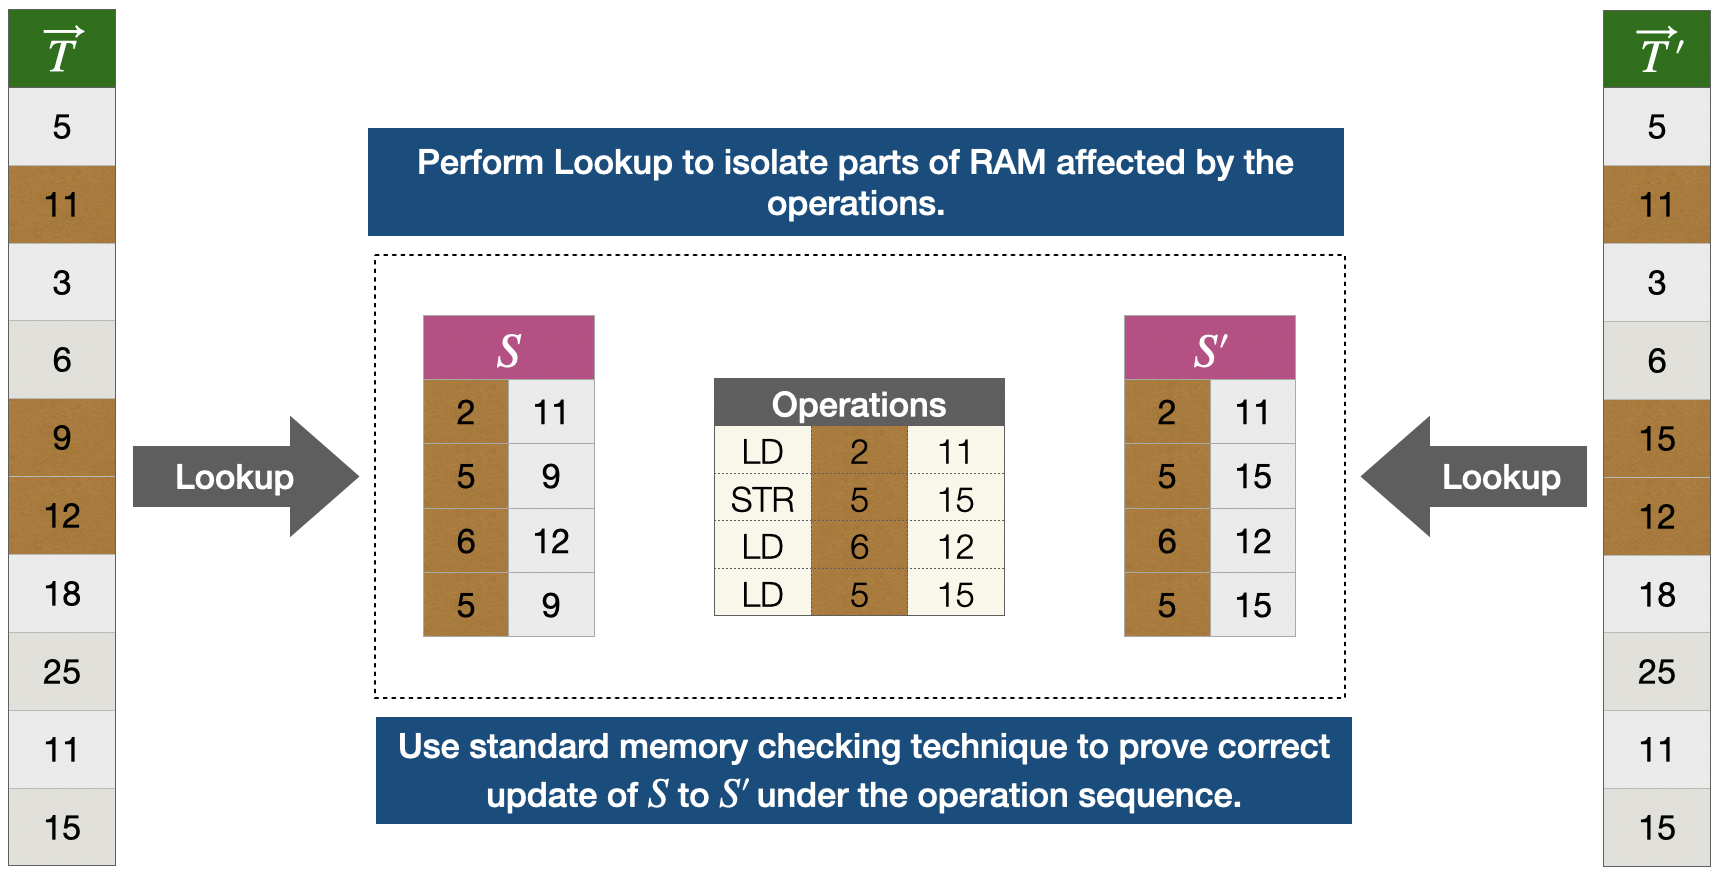
\includegraphics[width=\textwidth]{example-lookup}
		\caption{Isolating subtables using lookup argument}
		\label{fig:subtable-consistency}
	\end{subfigure}
	\begin{subfigure}{0.5\textwidth}
		\centering
		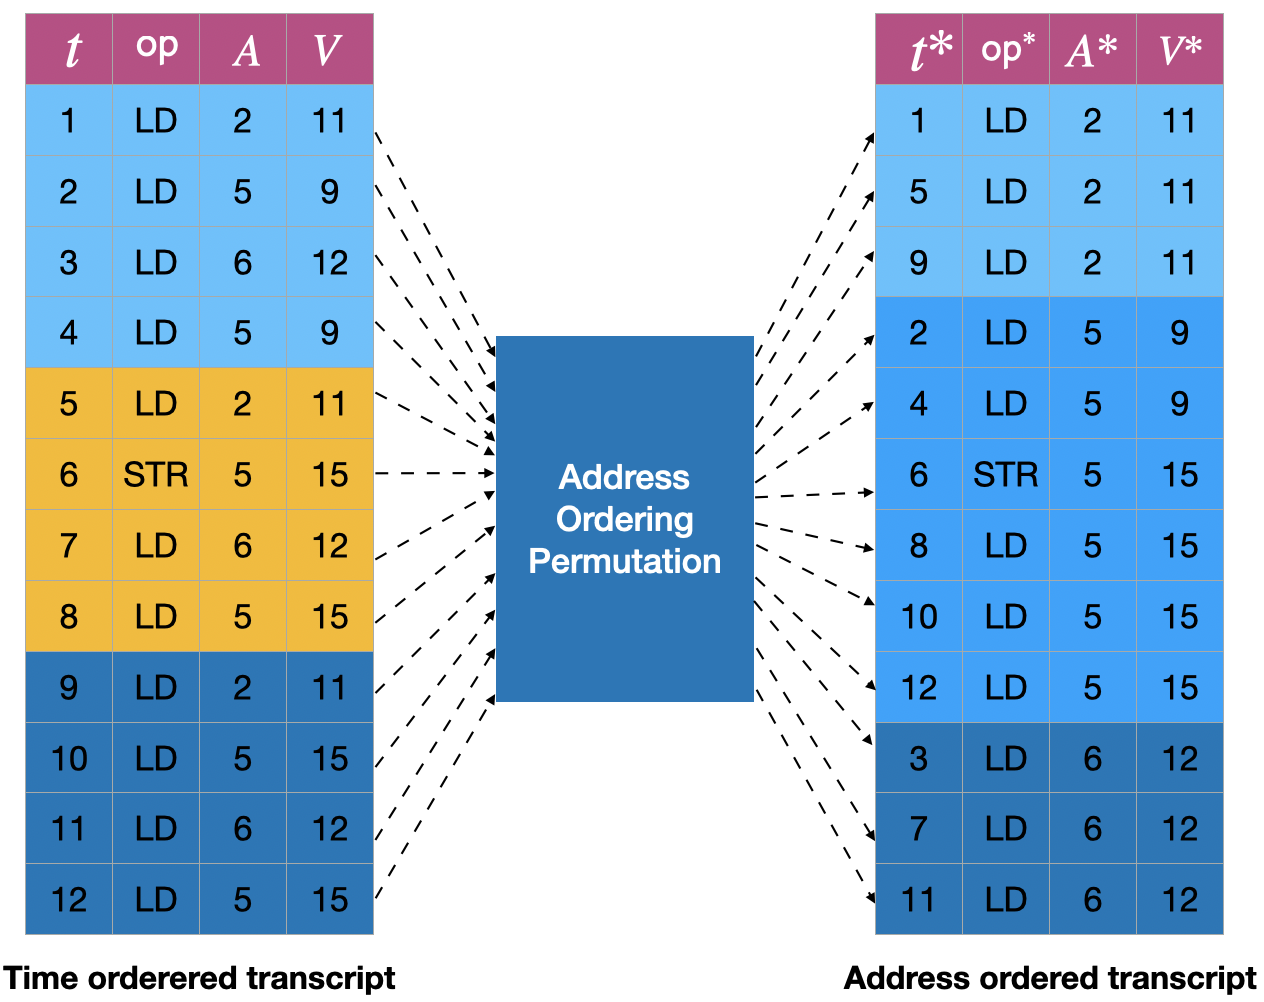
\includegraphics[height=0.3\textheight]{Address-ordered}
		\caption{Checking memory consistency using address ordering}
		\label{fig:permuted-transcripts}
	\end{subfigure}
\end{figure}

%
    \tikzset{
        table/.style={
            matrix of nodes,
            row sep=-\pgflinewidth,
            column sep=-\pgflinewidth,
            nodes={
                rectangle,
                draw=black,
                align=center
            },
            minimum height=1.5em,
            text depth=0.5ex,
            text height=1.5ex,
            nodes in empty cells,
%%
            every even row/.style={
                nodes={fill=gray!20}
            },
            column 1/.style={
                nodes={text width=2em}
            },
            row 1/.style={
                nodes={
                    fill=white,
                    text=black,
                    font=\bfseries
                },
            }
        }
    }

    \tikzset{
        MyArrow/.style={
            single arrow, draw=black, minimum width=10mm, minimum height=30mm, inner sep=0mm, single arrow head extend=1mm, double arrow head extend=1mm
        }
    }

    \begin{figure}[t]
        \centering
        %\subcaptionbox{Lookup to get sub-tables \label{fig:lookup}}[\textwidth]{
        \resizebox{0.8\textwidth}{0.3\textheight}{
        \begin{tikzpicture}
            %\draw[step=1.0,black,thin] (-5,-5) grid (5,5);
        \matrix (initial) [table,text width=2em, width=2cm] at (-5,1)
        {
            Idx & Val\\
            1  & 10 \\
            2  & 20 \\
            3  & 15 \\
            4  & 25 \\
            5  & 40 \\
            6 & 50 \\
            7 & 60 \\
        };

        \matrix (ops1) [table,text width=2em, width=2cm] at (0,0)
            {
            Op & Idx & Val \\
            \store  & 7 & 40 \\
            \load  & 1 & 10 \\
            \store & 3 & 20 \\
            \load  & 3 & 20 \\
        };


        \matrix (final) [table,text width=2em, width=2cm] at (5,1)
            {
            Idx & Val\\
            1  & 10 \\
            2  & 20 \\
            3  & 20 \\
            4  & 25 \\
            5  & 40 \\
            6 & 50 \\
            7 & 40 \\
        };


        % -------------------------------- Subtables ------------------------------------- %
        \matrix (stinitial) [table,text width=2em, width=2cm] at (-5,-5)
            {
            Idx & Val\\
            7 & 60 \\
            1 & 10 \\
            3 & 15 \\
            3 & 15 \\
        };

        \matrix (ops2) [table,text width=2em, width=2cm] at (0,-5)
            {
            Op & Idx & Val \\
            \store  & 7 & 40 \\
            \load  & 1 & 10 \\
            \store & 3 & 20 \\
            \load  & 3 & 20 \\
        };


        \matrix (stfinal) [table,text width=2em, width=2cm] at (5,-5)
            {
            Idx & Val\\
            7 & 40 \\
            1 & 10 \\
            3 & 20 \\
            3 & 20 \\
        };

            \draw (-5,3.6) node[above]  {\bf RAM $\vecT_0$};
            \draw (0, 1.6) node[above] {\bf Operations};
            \draw (5,3.6) node[above] {\bf RAM $\vecT_1$};
            \draw (-5, -3.4) node[above] {\bf $\vec{t}_0$};
            \draw (5, -3.4) node[above] {\bf $\vec{t}_1$};

            % lookup arrows
            \draw [-Latex, thick] (-4.25,-1.75) -- (-4.25,-3.25);
            \draw [-Latex, thick] (4.25, -1.75) -- (4.25, -3.25);
            \draw [fill=grey!30!white] (-2,-2) rectangle (2, -3) node[midway] {Lookup on indices 7,1,3,3};

            \draw (-2, -2.5) -- (-4.25, -2.5) (2, -2.5) -- (4.25, -2.5);
            \draw [-Latex, dashed] (-4, 0) -- (-1.6,0);
            \draw [-Latex, dashed] (1.6,0) -- (4,0);
            \draw [-Latex, dashed] (-4, -5) -- (-1.6,-5);
            \draw [-Latex, dashed] (1.6,-5) -- (4,-5);
        \end{tikzpicture}
        }
        \caption{Using lookup arguments to reduce the consistency check between large RAMs $\vecT_0$
        and $\vecT_1$ to that between small tables $\vec{t}_0$ and $\vec{t}_1$. It is seperately shown that RAMs $\vecT_0$ and
        $\vecT_1$ have identical values outside the involved indices. Figure ~\ref{fig:subtable-consistency} illustrates address
        ordered transcript to check consistency of $\vec{t}_0$ and $\vec{t}_1$.}
        \label{fig:subtable-lookup}
        \end{figure}

        \begin{figure}[htbp]
            \centering
            \resizebox{0.8\textwidth}{0.4\textheight}{
        \begin{tikzpicture}
        % ------------------------------------------------------------------------------------------- %
            %\draw[step=1.0,black,thin] (-5,-5) grid (5,5);
        \matrix (trts) [table,text width=2em] at (-4,0)
            {
            Ts & Op & Idx & Val\\
            1 & \store & 7 & 60 \\
            2 & \store & 1 & 10 \\
            3 & \store & 3 & 15 \\
            4 & \store & 3 & 15 \\
            5 & \store  & 7 & 40 \\
            6 & \load  & 1 & 10 \\
            7 & \store & 3 & 20 \\
            8 & \load  & 3 & 20 \\
            9 & \load & 7 & 40 \\
            10 & \load & 1 & 10 \\
            11 & \load & 3 & 20 \\
            12 & \load & 3 & 20 \\
        };

        \matrix (trts) [table,text width=2em, width=2cm] at (4,0)
            {
            Ts & Op & Idx & Val\\
            2 & \store & 1 & 10 \\
            6 & \load & 1 & 10 \\
            10 & \load & 1 & 10 \\
            3 & \store & 3 & 15 \\
            4 & \store  & 3 & 15 \\
            7 & \store  & 3 & 20 \\
            8 & \load & 3 & 20 \\
            11 & \load  & 3 & 20 \\
            12 & \load & 3 & 20 \\
            1 & \store & 7 & 60 \\
            5 & \store & 7 & 40 \\
            9 & \load & 7 & 40 \\
        };

            \path (-2.1,0) -- (1.9, 0)  node[midway, MyArrow, text width=3cm, align=center] {Address-sorting permutation};
            \draw (-4, 4.3) node[above] {\bf \small Time ordered transcript ($\mathsf{tr}$)};
            \draw (4, 4.3) node[above] {\bf \small Address ordered transcript ($\mathsf{tr}^\ast$)};

        \end{tikzpicture}
            }
            \caption{Address ordered transcript for checking consistency of tables $\vec{t}_0$ and $\vec{t}_1$
                with respect to the operation sequence in Figure \ref{fig:subtable-lookup}. On the transcript
            $\mathsf{tr}^\ast$, one checks that the load instructions return the same value as the preceeding
            instruction if their indices are the same.}

        \label{fig:subtable-consistency}
    \end{figure}

\noindent{\bf Our Contributions}: (Summarise later)

\section{Related Work}\label{sec:rel-work}

\section{Preliminaries}\label{sec:prelims}
%    
Throughout the paper, we assume a bilinear group generator $\bg$ which on input $\lambda$ outputs
parameters for the protocols. Specifically $\bg(1^\secp)$ outputs $(\F,\Gone,\Gtwo,\GT, e, g_1, g_2,g_t)$
where:
\begin{itemize}[leftmargin=2em, label=-]
	\item $\F=\Fp$ is a prime field of super-polynomial size in $\lambda$, with $p=\lambda^{\omega(1)}$.
	\item $\Gone,\Gtwo$ and $\GT$ are groups of order $p$, and $e$ is an efficiently computable non-degenerate
	pairing $e:\Gone\times \Gtwo\rightarrow \GT$.
	\item Generators $g_1,g_2$ are uniformly chosen from $\Gone$ and $\Gtwo$ respectively and $g_t=e(g_1,g_2)$.
\end{itemize}
We write groups $\Gone$ and $\Gtwo$ additively, and use the shorthand notation $\gone{x}$ and $\gtwo{x}$
to denote group elements $x\cdot g_1$ and $x\cdot g_2$ respectively for $x\in \F$. We will implicity assume
that all the setup algorithms for the protocols invoke $\bg$ to generate descriptions of groups and fields
over which the protocol is instantiated. We will use the notation
$[n]$ to denote the set of integers $\{1,\ldots,n\}$.

\noindent{\bf Security Model}: We describe public-coin interactive protocols, involving a prover and a verifier,
where both the parties have access to a structured reference string (SRS). The SRS in our protocol consists of
encodings of monomials of the form $\left\{\gone{x^i}\}_{a\leq i\leq b}$, $\left\{\gtwo{x^i}\}_{c\leq i\leq d}$
for $x$ chosen uniformly from $\F$ and $a,b,c,d$ are bounded by some polynomial in $\lambda$. It then follows
from ~\cite{EPRINT:BowGabMie17} that such an SRS can be generated using a universal and updatable setup requiring
only one honest participant. In practice, this gives us a far superior security model to the one requiring a fully
trusted setup. We use $\srs = (\srs_1,\srs_2)$ to denote the structured reference string of the above form. We say
that the $\srs$ has degree $Q$ if all the elements of $\srs_i$, $i=1,2$ are of the form $[f(x)]_i$ for a
polynomial $f\in \F_{<Q}[X]$.\smallskip


\noindent{\bf Algebraic Group Model}: We analyse our protocols in the Algebraic Group Model (AGM) introduced
in ~\cite{C:FucKilLos18}. We consider {\em algebraic adversaries} $\Adv$, which in our SRS-based protocol means
an efficient algorithm satisfying the following:
\begin{itemize}[leftmargin=1em]
	\item For $i\in \{1,2\}$, whenever $\Adv$ outputs an element $A\in \G_i$, it also outputs a vector $\vec{v}$
	over $\F$ such that $A=\langle \vec{v},\srs_i\rangle$.
\end{itemize}
Algebraic group model is a useful framework for obtaining succinct arguments of knowledge (SNARKs) from interactive
protocols described as {\em polynomial protocols} ~\cite{Gabizon2019PLONKPO}. Informally, the prover's messages in
a polynomial protocol are low degree polynomials, and the verifier accepts or rejects by checking certain identities
over polynomials output by the prover and possibly public polynomials known to the verifier. A polynomial protocol can
be compiled into a succinct argument of knowledge by using an extractable polynomial commitment scheme, which allows a
prover to send commitments to polynomials, and later send evaluation proofs for the same to enable the verifier to probabilistically
check polynomial identities at random points of $\F$. We refer the reader to ~\cite[Section 4.2]{Gabizon2019PLONKPO} for details
on polynomial protocols and their compilation to SNARKs in the algebraic group model.

\subsection{KZG Commitment Scheme}
\label{sec:KZG}
We use the $\kzg$ commitment scheme introduced in ~\cite{AC:KatZavGol10} which satisfies succinctness, completeness and knowledge-soundness (extractability)
in the algebraic group model, while additionally featuring a universal and updatable setup. We denote the $\kzg$ scheme by the tuple
of $\ppt$ algorithms $(\KZGsetup$,$\KZGcommit$, $\KZGopen$, $\KZGverify)$ as defined below.
%We then establish the isomorphism of the KZG polynomial commitment scheme as a vector commitment scheme.
\begin{definition}[KZG Polynomial Commitment Scheme]
	Let $(\F,\Gone,\Gtwo,\GT, e, g_1, g_2, g_t)$ be output of bilinear group generator $\bg(1^\secp)$ for security parameter $\secp$.
	The KZG polynomial commitment scheme is defined as follows:
	\begin{itemize}[leftmargin=1em]
		\item $\KZGsetup$ on input $(1^\secp,d)$, where $d$ is the degree bound, outputs
		$\srs = \{\eltone{\tau},\ldots,\eltone{\tau^d}\}$ ,$\{\elttwo{\tau},\ldots,\elttwo{\tau^d}\}$.
		\item $\KZGcommit$ on input $(\srs,p(X))$, where $p(X) \in \F_{\leq d}[X]$, outputs $C=\eltone{p(\tau)}$
		\item $\KZGopen$ on input $(\srs,p(X),\alpha)$, where $p(X) \in \F_{\leq d}[X]$ and $\alpha\in \F$, outputs $(v, \pi)$ such that $v=p(\alpha)$ and $\pi=\eltone{q(\tau)}$, for
		\[ q(X)=\frac{p(X)-p(\alpha)}{X-\alpha} \]
		\item $\KZGverify$ on input $(\srs,C,\alpha,v,\pi)$, outputs $1$ if the following equation holds, and $0$ otherwise.
		\[ e(C-v, \elttwo{\tau}) = e(\pi, \elttwo{\tau-\alpha}) \]
	\end{itemize}
\end{definition}

We also assume (w.l.o.g) analogues of $\KZGcommit$, $\KZGopen$ and $\KZGverify$ defined over the group $\Gtwo$.
We shall use the (non-standard) notation $[p(X)]_i$ to denote $[p(\tau)]_i$ for $i\in \{1,2\}$.
This allows us a convenient shorthand for referring to ``commitment of the polynomial $p(X)$'' in group $\G_i$.
Our protocols also use batched KZG proofs to show that polynomial $p(X)$ satisfies $p(\alpha_i)=v_i$ for $i\in [n]$. Let
$\vec{\alpha}=(\alpha_1,\ldots,\alpha_n)$
denote the vector of evaluation points and $\vec{v}=(v_1,\ldots,v_n)$ denote the vector of claimed evaluations. Then the batched
version of $\KZGopen$ is described as follows:
\begin{itemize}[leftmargin=1em]
	\item $\KZGopen$ on input $(\srs,p(X),\vec{\alpha})$, where $p(X) \in \F_{\leq d}[X]$ and $\vec{\alpha}\in\F^n$,
	outputs $(\vec{v}, \pi)$ with $\vec{v}\in \F^n$ such that $v_i=p(\alpha_i)$ and $\pi=\eltone{q(\tau)}$ where
	\[ q(X)=\frac{p(X)-r(X)}{a(X)} \]
	In the above, $a(X)=(X-\alpha_1)\cdots(X-\alpha_n)$, while $q(X)$ and $r(X)$ are the quotient and remainder polynomials when
	 $p(X)$ is divided by $a(X)$.
	%Note that the polynomials $a(X)$ and $r(X)$ can be computed by the verifier since $\{\alpha_i,v_i\}_{i\in [n]}$ are known and
	%$a(X)=(X-\alpha_1)\cdots(X-\alpha_n)$ and $r(\alpha_i)=v_i$ for all $i\in [n]$ such that $0\leq \deg(r(X)) \leq n$.
	\item $\KZGverify$ on input $(\srs,C,\vec{\alpha},\vec{v},\pi)$, outputs $1$ if the following equations holds, and $0$ otherwise.
	\begin{align*}
		e(C-\eltone{r(\tau)}, \elttwo{\tau}) &= e(\pi, \elttwo{a(\tau)})
	\end{align*}
	Here, the verifier interpolates the polynomial $r(X)\in \F_{<n}[X]$ such that $r(\alpha_i)=v_i$.
\end{itemize}

%\begin{definition}[KZG Polynomial Commitment Scheme \textcolor{red}{degree check included}]
%    Let $(p,\Gone,\Gtwo,\GT, e, \eltone{1},\elttwo{1})$ be a bilinear group. The KZG polynomial commitment scheme is defined as follows: 
%    \begin{itemize}
%	        \item $\KZGsetup$ on input $(1^\lambda,d)$, where $\lambda$ is the security parameter and $d$ is the degree bound, outputs $\srs = \{ \eltone{\tau},\ldots,\eltone{\tau^d},\elttwo{\tau},\ldots,\elttwo{\tau^d}\}$
%	        \item $\KZGcommit$ on input $(\srs,p(X))$, where $p(X) \in \F_{\leq d}[X]$, outputs $C=\eltone{p(X)}:=\eltone{p(\tau)}$
%	        \item $\KZGopen$ on input $(\srs,p(X),\alpha)$, where $p(X) \in \F_{\leq d}[X]$ and $\alpha\in \F$, outputs $(v, \pi)$ such that $v=p(\alpha)$ and $\pi=\Comtwo{q(X)}:=\elttwo{q(\tau)}$, for
%	        \[ q(X)=\frac{p(X)-p(\alpha)}{X-\alpha} \]
%	        \item $\KZGverify$ on input $(\srs,C,\deg,\alpha,v,\pi)$, outputs $1$ if the following equation holds, and $0$ otherwise.
%	        \[ e(C-v, \elttwo{\tau}) = e(\pi, \elttwo{\tau-\alpha}) \]
%	        { \color{teal} \moumita{var 3.}
%		        Degree check has not been added. With degree check, $\pi$ is modified with
%		        \[ q(X)=X^{d-\deg(p(X))+2}\frac{p(X)-p(\alpha)}{X-\alpha} \]
%		        and the verification equation if modified as 
%		        \[ e(C-v, \elttwo{\tau}^{d-\deg+2}) = e(\pi, \elttwo{\tau-\alpha}) \]
%		        } %stays unchanged from var 1
%	    \end{itemize}
%\end{definition}
\nitin{Defer the commitment to vectors to where we need it}
\begin{comment}
\paragraph{Vector Commitment Scheme.} We note that there is a natural isomorphism between the set of vectors of length $n$ and polynomials of degree $n-1$, where any vector $\abf=(a_1,\ldots,a_n) \in \F^n$ has a natural equivalent representation as a polynomial $a(X)=a_1\lambda_1(X)+\ldots,a_n\lambda_n(X)$, where $\{\lambda_i(X)\}_{i\in [n]}$ is basis of $\F_{\leq n-1}[X]$. Hence, when we use the KZG polynomial commitment scheme for a vector $\abf=(a_1,\ldots,a_n) \in \F^n$, we can output the commitment as $\KZGcommit(\srs,a(X))$, where $a(X)=a_1\lambda_1(X)+\ldots,a_n\lambda_n(X)$.


Now, for vectors of length $n$, we consider the basis $\{\lambda_i(X)\}$ to be the langrange basis with respect to the set consisting of $n^{th}$ roots of unity $\doubleH=\{\omega,\ldots,\omega^n\}$. The lagrange basis helps us use the property that, for some $i\in [n]$ and a value $\alpha$, $a(\omega^i)=a_i=\alpha$ if and only if there exists a polynomial $W(X)$ such that $W(X)=\frac{a(X)-\alpha}{X-\omega^i}$. 
\end{comment}
%Throughout the draft, for $\abf\in \F^n$, we use $\Comone{.}$ to denote $\KZGcommit(\srs,\abf)$ for vectors of length $n$, using the langrange polynomial basis $\{\lambda_i(X)\}$, with respect to the $n^{th}$ root of unity $\omega$, and for $\bbf \in \F^m$, we use $\Comtwo{.}$ to denote $\KZGcommit(\srs,\bbf)$ for vectors of length $m$, using the langrange polynomial basis $\{\mu_i(X)\}$, with respect to the $m^{th}$ root of unity $\nu$.

\section{Model for RAM}\label{sec:model-for-ram}
In this section, we briefly review and formalize existing memory-checking techniques to ensure
correctness of RAM operations. The formal definitions for various relations involved in memory checking
will be used to describe polynomial protocol for RAM in Appendix~\ref{sec:poly-proto-ram-app}.

\subsection{Correctness of RAM Update}\label{subsec:ram-update}
The versatility of the RAM primitive stems from its updatability. While a load operation leaves the RAM unchanged, the store operation
updates the value in the RAM associated with the referenced index. We model the update via the function
$\Rupd{I}$ which takes RAM $\vecT\in \RAM{I}{n}$, operation
$o=(\op,a,v)\in \RAMOp{I}$ as inputs and returns an updated RAM $\vecT'\in \RAM{I}{n}$.
The updated RAM $\vecT'=\Rupd{I}(\vecT,o)$ satisfies
$\vecT'=\vecT$ if $\op=0$ while for $\op=1$ it satisfies $\vecT'[\,a\,]=v$  and $\vecT'[\,x\,]=\vecT[\,x\,]$ for $x\neq a$. The central problem
in verifiable RAM protocols is to establish that a sequence of operations $\vec{o}=(o_1,\ldots,o_m)$ are correct with
respect to the initial RAM state $\vecT$ and the final RAM state $\vecT'$. This involves ensuring
that all load operations read the value which is consistent with updates to the RAM as a result of preceding
store operations, and that $\vecT'$ is the final state. We say that an operation $o=(\op,a,v)$ is {\em load-consistent}
with respect to RAM $\vec{T}$ if $v=\vecT[a]$ whenever $o$ is a load operation (store operations are vacuously defined to be load-consistent).
We formally define the notion of consistency below:

\begin{definition}[Consistent Operations]\label{defn:consistent-operations}
    Let $n\in \N$ and $\vecT,\vecT'\in \RAM{I}{n}$ for some index set $\setind$. We say that a sequence of operations
    $\vec{o}=(o_1,\ldots,o_k)\in \RAMOp{I}^k$ over $\setind$ is {\em consistent} with RAM states
    $\vecT,\vecT'$ if for all $i\in [k]$, $\vecT_{i}=\Rupd{I}(\vecT_{i-1},o_i)$ and operation $o_i$ is load-consistent with respect to $\vecT_{i-1}$. Here
    we assume $\vecT_0=\vecT$ and $\vecT_k=\vecT'$.
\end{definition}

For $m,n\in \N$, let $\LRAM{I}{m}{n}$ denote the language consisting of tuples $(\vecT,\vec{o},\vecT')$ with $\vecT,\vecT'\in \RAM{I}{n}$ and $\vec{o}\in (\RAMOp{I})^m$
such that $\vec{o}$ is consistent with $\vecT,\vecT'$.
Next, we formalize the folklore technique of checking correctness of RAM operations
using {\em address-ordered transcripts}.

\subsection{Consistency Check via Transcripts}\label{subsec:transcripts}
A {\em transcript} is time-stamped sequence of operations executed on a RAM.
More formally, given a RAM $\vecT=(\vec{a},\vec{v})\in \RAM{I}{n}$,
operation sequence $\vec{o}=(o_1,\ldots,o_m)$ with $o_i=(\bar{\op_i},\bar{a}_i,\bar{v}_i)\in \RAMOp{I}$ and RAM $\vecT'=(\vec{a}', \vec{v}')\in \RAM{I}{n}$,
the {\em time ordered transcript} for the tuple $(\vecT,\vec{o},\vecT')$ is given by the table $\tr$ with $k=2n+m$ rows and four columns
$\tr = (\vec{t},\vec{\op},\vec{A},\vec{V})$  defined as follows: (i) $\vec{t}=\setind_{k}=(1,\ldots,k)$,
(ii) $\vec{\op}=0^n||(\bar{\op}_1,\ldots,\bar{\op}_m)||0^n$,
(iii) $\vec{A}=\vec{a}||(\bar{a}_1,\ldots,\bar{a}_m)||\vec{a}'$ and
(iv) $\vec{V}=\vec{v}||(\bar{v}_1,\ldots,\bar{v}_m)||\vec{v}'$. The $i^{th}$ row of the table $\tr$ is
$(t_i,\op_i,A_i,V_i)$ for $i\in [k]$. The first $n$ records in $\tr$ correspond to the contents of $\vecT$,
the next $m$ records correspond to the operations in $\vec{o}$ and final $n$
records correspond to contents of $\vecT'$. The timestamp column $\vec{t}$ is added to order operations with the same index.
Notationally, we write $\tr=\TOT(\vecT,\vec{o},\vecT')$.

We call a transcript $\tr=(\vec{t},\vec{\op},\vec{A},\vec{V})$ to be {\em address ordered} if $A_i\leq A_{i+1}$ for $i\in [k-1]$ and
$t_i < t_{i+1}$ whenever $A_i=A_{i+1}$. For a transcript $\tr=(\vec{t},\vec{\op},\vec{A},\vec{V})$ with $k$ records and a
permutation $\sigma:[k]\rightarrow [k]$, we use $\sigma(\tr)$ to denote the transcript
$(\sigma(\vec{t}),\sigma(\vec{\op}),\sigma(\vec{A}),\sigma(\vec{V}))$
obtained by permuting the records of $\tr$ according to the permutation $\sigma$.
An address ordered transcript for tuple $(\vecT,\vec{o},\vecT')$ is defined as $\tr^\ast=\sigma(\tr)$ where $\tr=\TOT(\vecT,\vec{o},\vecT')$ and $\sigma$ is
a permutation such that $\tr^\ast$ is address ordered. We denote it by $\tr^\ast=\AOT(\vecT,\vec{o},\vecT')$.
We say that an address ordered transcript $\tr=(\vec{t},\vec{\op},\vec{A},\vec{V})$ satisfies {\em load-store correctness}
if for all pairs of consecutive records $(t_i,\op_i,A_i,V_i)$ and $(t_{i+1},\op_{i+1},A_{i+1},V_{i+1})$ we have $V_{i+1}=V_i$
whenever $\op_{i+1}=0$ (load operation) and
$A_i=A_{i+1}$, i.e, a load operation does not change the value at an index.
We formally state the folklore technique for enforcing memory consistency in our setting.
\begin{lemma}\label{lem:consistency-check}
Let $\F$ be a finite field, $m,n\in \N$ be positive integers and $\setind\subseteq \F$. Then $(\vecT,\vec{o},\vecT')\in \LRAM{I}{n}{m}$ if and only if
    the address ordered transcript $\tr^\ast=\AOT(\vecT,\vec{o},\vecT')$ satisfies load-store correctness.
\end{lemma}

The consistency check in Lemma \ref{lem:consistency-check} can be encoded as an arithmetic circuit of size $\wt{O}(m+n)$, thus
yielding an argument of knowledge for the language $\LRAM{I}{n}{m}$ with prover complexity quasi-linear in
$m+n$. For completeness, we present a self-contained argument of knowledge for
$\LRAM{I}{m}{m}$ ($m=n$) based on the ``polynomial protocol'' framework defined in ~\cite{Gabizon2019PLONKPO}.



\begin{comment}
\begin{enumerate}[leftmargin=2em]
\item $\prover\rightarrow\verifier$: For the transcript $\tr^\ast=(\vec{t^\ast},\vec{\op^\ast},\vec{A^\ast},\vec{V^\ast})$,
the prover computes encoding polynomials $\wt{\tr^\ast}=({t^\ast}(X),\op^\ast(X), A^\ast(X),V^\ast(X))$. Next, the prover
computes sets $I_1$ and $I_2$ as in Section \ref{subsec:encoded-relations}, and then computes polynomials
$Z_b(X)=\prod_{i\in I_b}(X-\omega^i)$ for $b=1,2$.
The prover also interpolates polynomials $\delta^\ast_A(X)$ and $\delta^\ast_T(X)$ satisfying
$\delta^\ast_A(\omega^i) = A^\ast_{i+1} - A^\ast_i$ for $i\in I_1$ and $\delta^\ast_T(\omega^i)=t^\ast_{i+1}-t^\ast_i$ for $i\not\in I_1$.
The prover sends all the above polynomials to the verifier.
\item $\verifier$ computes: The verifier checks relations (C1)-(C6) in Lemma \ref{lem:addr-ordered-transcript}. The range constraints
in (C7) can be verified using polynomial protocols in sub-vector lookup arguments such as Caulk+ ~\cite{EPRINT:PosKat22}, CQ
~\cite{EPRINT:EagFioGab22}.
\end{enumerate}


\subsection{Succinct Argument for Verifiable RAM}\label{subsec:succ-args}
Polynomial protocols can be compiled into succinct arguments of knowledge using an extractable polynomial commitment scheme. At a
high level the compilation involves the prover sending ``commitments'' to the message polynomials, whereas the verifier checks
the polynomial identities probabilistically by requesting evaluation proofs of the polynomials at random points.
We complile the polynomial protocol for RAM to a succinct argument of knowledge in the Algebraic Group Model (AGM)
 using $\kzg$ as the extractable polynomial commitment scheme. We also leverage homomorphism of $\kzg$ scheme
to avoid sending commitments and evaluations for polynomials which are linear combinations of previously committed polynomials.
We now present an argument for verifiable RAM, which combines the polynomial protocols in this section, and instantiates
them using $\kzg$ commitments. We make standard optimisations of batching several identity checks into one where applicable.
Let $\srs=\{\gone{\tau^i},\gtwo{\tau^i}\}_{i=0}^d$
denote the $\kzg$ setup parameters for degree $d\geq k$ for the bilinear group $\mathsf{BG}=(\Gone,\Gtwo,\gone{1},\gtwo{1},e)$. Let
$\F=\F_p$ be the finite field where $p$ is the order of the groups.


\begin{figure}[t]
\begin{subfigure}{\linewidth}
\centering
{\footnotesize
\begin{enumerate}[leftmargin=1em]
    \item $\prover\rightarrow\verifier$: Send polynomial commitments $\gone{a(X)}$, $\gone{v(X)}$, $\gone{a'(X)}$, $\gone{v'(X)}$,
    $\gone{\bar{\op}(X)}$, $\gone{\bar{a}(X)}, \gone{\bar{v}(X)}$, $\gone{\op(X)}$, $\gone{A(X)}$, $\gone{V(X)}$, $\gone{t^\ast(X)}$,
    $\gone{\op^\ast(X)}$, $\gone{A^\ast(X)}$, $\gone{V^\ast(X)}$, $\gone{\delta_A^\ast(X)}$, $\gone{\delta_T^\ast(X)}$.
    \item $\verifier\rightarrow\prover$: Send $\alpha,\beta,\gamma\gets \F$.
    \item $\prover$ computes: Compute sets $I_1=\{i\in [k]: A^\ast_i\neq A^\ast_{i+1}\}$, and $I_2=[k]\setminus I_1$. Next, compute
    polynomials:
    \begin{align*}
        &Z_1(X)=\prod_{i\in I_1}(X-\omega^i),\quad Z_2(X)=\prod_{i\in I_2}(X-\omega^i), \\
        &H(X) = \begin{bmatrix} 1 & \gamma & \gamma^2 \end{bmatrix}
        \begin{bmatrix}
            a(X) & v(X) & 0 \\
            a'(X) & v'(X) & 0 \\
            \bar{a}(X) & \bar{v}(X) & \bar{\op}(X)
        \end{bmatrix}
        \begin{bmatrix}
        1 \\
        \beta \\
        \beta^2
        \end{bmatrix}, \\
        &G(X) = A(X) + \beta V(X) + \beta^2 \op(X), \\
        &Q(X) = \big(H(X^3) - G(X) - \gamma G(\omega^m X) - \gamma^2 G(\omega^{2m} X)\big)/Z(X), \\
        &f(X) = G(X) + \beta^3 t(X),\, g(X) = A^{\ast}(X) + \beta V^{\ast}(X) + \beta^2 \op^{\ast}(X) + \beta^3 t^{\ast}(X), \\
        &z(X) = \sum_{i=1}^k \lambda_i(X)\prod_{j=1}^{i-1} (\alpha - g(\omega^j))/(\alpha - f(\omega^j)), \\
        &Q_1(X) = \frac{1}{\mathbb{Z}_\setH(X)}\Big( (\alpha - g(X))z(\omega X) - (\alpha - f(X))z(X) \\
        &\qquad\qquad + \beta Z_2(X)(A^\ast(\omega X) - A^\ast(X) - \delta_A^\ast(X))\Big), \\
        &Q_2(X) = \frac{1}{Z_2(X)}\Big((A^\ast(\omega X) - A^\ast(X))
         + \beta(t^\ast(\omega X) - t^\ast(X)-\delta_T^\ast(X)) \\
        &\qquad\qquad + \beta^2 (\op^\ast(X) - 1)(V^\ast(\omega X) - V^\ast(X))\Big)
    \end{align*}
    \item $\prover\rightarrow \verifier$: Send $\gone{Z_1(X)}$, $\gone{Z_2(X)}$, $\gone{Q(X)}$, $\gone{z(X)}$,
    $\gone{Q(X)}$, $\gone{Q_1(X)}$, $\gone{Q_2(X)}$.
    \item $\verifier\rightarrow\prover$: $s\gets \F$.
    \item $\prover\rightarrow\verifier$: Send evaluations $\val{Z_1}{s}=Z_1(s)$, $\val{Z_2}{s}=Z_2(s)$,
    $\val{G}{s}=G(s)$, $\val{Q}{s}=Q(s)$, $\val{Z}{s}=Z(s)$, $\val{A^\ast}{s}=A^\ast(s)$, $\val{V^\ast}{s}=V^\ast(s)$,
    $\val{\op^\ast}{s}=\op^\ast(s)$, $\val{t}{s}=t(s)$, $\val{t^\ast}{s}=t^\ast(s)$, $\val{z}{s}=z(s)$, $\val{Q_1}{s}=Q_1(s)$,
    $\val{Q_2}{s}=Q_2(s)$, $\val{H}{s^3}=H(s^3)$, $\val{G}{\omega^m s}=G(\omega^m s)$, $\val{\delta^\ast_A}{s}=\delta_A^\ast(s)$,
    $\val{\delta_T^\ast}{s}=\delta_T^\ast(s)$
    $\val{G}{\omega^{2m} s}=G(\omega^{2m} s)$,
    $\val{A^\ast}{\omega s}=A^\ast(\omega s)$, $\val{V^\ast}{\omega s}=V^\ast(s)$, $\val{t^\ast}{\omega s}=t^\ast(\omega s)$,
    $\val{z}{\omega s}=z(\omega s)$, $\val{A^\ast}{\omega}=A^\ast(\omega)$.

    \item $\verifier\rightarrow\prover$: Send $r \gets \F$.
    \item $\prover$ computes: Compute batched $\kzg$ proofs:
    \begin{alignat*}{3}
        &P_1 && &\quad=\quad  && &Z_1+r Z_2 + r^2 G + r^3 Q + r^4 Z + r^5 A^{\ast} + r^6 V^{\ast} + r^7 \op^{\ast} \\
        & && & && &\quad  + r^8 t + r^9 t^{\ast} + r^{10} z + r^{11} Q_1 + r^{12} Q_2 + r^{13} \delta_A^{\ast} + r^{14} \delta_T^{\ast} \\
        &P_2 && &\quad=\quad && &A^{\ast} + r V^{\ast} + r^2 z \\
        &\Pi_s && &\quad=\quad && &\kzgprove(P_1, s) \\
        &\Pi_{\omega s} && &\quad=\quad && &\kzgprove(P_2, \omega s) \\
        &\Pi_{s^3} && &\quad=\quad && &\kzgprove(H, s^3) \\
        &\Pi_{\{\omega^m s, \omega^{2m} s\}} && &\quad=\quad && &\kzgprove(G, (\omega^m s, \omega^{2m} s))
    \end{alignat*}
    \item $\prover\rightarrow \verifier$: Send $\Pi_s,\Pi_{\omega s}, \Pi_{s^3},\Pi_{\{\omega^m s, \omega^{2m} s\}}$ and
    $\val{H}{s^3},\val{G}{\omega^m s}, \val{G}{\omega^{2m} s}$.

    \item $\verifier$ computes: Compute commitments and evaluations for linear combinations.
    \begin{align*}
        \gone{G(X)} &= \gone{A(X)}+\beta\gone{V(X)}+\beta^2\gone{\op(X)}, \\
        \gone{H(X)} &= \begin{bmatrix} 1 & \gamma & \gamma^2 \end{bmatrix}
        \begin{bmatrix}
            \gone{a(X)} & \gone{v(X)} & \gone{0} \\
            \gone{a'(X)} & \gone{v'(X)} & \gone{0} \\
            \gone{\bar{a}(X)} & \gone{\bar{v}(X)} & \gone{\bar{\op}(X)}
        \end{bmatrix}
        \begin{bmatrix}
            1 \\
            \beta \\
            \beta^2
        \end{bmatrix}, \\
        \gone{P_1(X)} &= \gone{Z_1(X)}+r \gone{Z_2(X)} + r^2 \gone{G(X)} + r^3 \gone{Q(X)} + r^4 \gone{Z(X)} + r^5 \gone{A^{\ast}(X)} \\
         &\qquad + r^6 \gone{V^{\ast}(X)} + r^7 \gone{\op^{\ast}(X)} + r^8 \gone{t(X)} + r^9 \gone{t^{\ast}(X)} + r^{10} \gone{z(X)} \\
         &\qquad + r^{11} \gone{Q_1(X)} + r^{12} \gone{Q_2(X)} + r^{13} \gone{\delta_A^{\ast}(X)} + r^{14} \gone{\delta_T^{\ast}(X)}, \\
        \gone{P_2(X)} &= \gone{A^\ast(X)} + r\gone{V^\ast(X)} + r^2\gone{z(X)},\\
        \val{P_1}{s} &= \val{Z_1}{s}+r \val{Z_2}{s} + r^2 \val{G}{s} + r^3 \val{Q}{s} + r^4 \val{Z}{s} + r^5 \val{A^{\ast}}{s} \\
         &\qquad + r^6 \val{V^{\ast}}{s} + r^7 \val{\op^{\ast}}{s} + r^8 \val{t}{s} + r^9 \val{t^{\ast}}{s} + r^{10} \val{z}{s} \\
         &\qquad + r^{11} \val{Q_1}{s} + r^{12} \val{Q_2}{s} + r^{13} \val{\delta_A^{\ast}}{s} + r^{14} \val{\delta_T^{\ast}}{s}, \\
        \val{P_2}{\omega s} &= \val{A^\ast}{s} + r\val{V^\ast}{s} + r^2\val{z}{s}. \\
        \val{g}{s} &= \val{A^\ast}{s} + \beta \val{V^\ast}{s} + \beta^2 \val{\op^\ast}{s} + \beta^3 \val{t^\ast}{s}, \\
        \val{f}{s} &= \val{G}{s} + \beta^3 \val{t}{s}.
    \end{align*}

    \item $\verifier$ checks polynomial identities at $s$:
    \begin{alignat*}{3}
        &\val{Q}{s}\val{Z}{s} && &\quad \stackrel{?}{=}\quad  && &\val{H}{s^3} - \val{G}{s} - \gamma \val{G}{\omega^m s} - \gamma^2 \val{G}{\omega^{2m} s} \\
        &\val{Q_1}{s}(s^k-1) && &\quad \stackrel{?}{=}\quad && &(\alpha - \val{g}{s})\val{z}{\omega s} - (\alpha - \val{f}{s})\val{z}{s}
        +\beta \val{Z_2}{s}(\val{A^\ast}{\omega s}-\val{A^\ast}{s}-\val{\delta_A^\ast}{s}). \\
        &\val{Q_2}{s}\val{Z_2}{s} && &\quad \stackrel{?}{=}\quad && &(\val{A^\ast}{\omega s} - \val{A^\ast}{s}) + \beta (\val{t^\ast}{s} - \val{t}{s} - \val{\delta}{s}) \\
        & && & && &\qquad + \beta^2 (\val{\op^\ast}{s} - 1)(\val{V^\ast}{\omega s}-\val{V^\ast}{s}) \\
        &\val{Z_1}{s}\val{Z_2}{s} && &\quad \stackrel{?}{=}\quad && &s^k - 1 \\
    \end{alignat*}
    \item $\verifier$ checks evaluation proofs:
    \begin{alignat*}{3}
        &\kzgverify(\gone{P_1(X)},\val{P_1}{s},s, \Pi_s) && &\quad\stackrel{?}{=}\quad && &1 \\
        &\kzgverify(\gone{P_2(X)},\val{P_2}{\omega s},\Pi_{\omega s}) && &\quad\stackrel{?}{=}\quad && &1 \\
        &\kzgverify(\gone{H(X)},\val{H}{s^3},\Pi_{s^3}) && &\quad\stackrel{?}{=}\quad && &1 \\
        &\kzgverify(\gone{G(X)},(\val{G}{\omega^m s},\val{G}{\omega^{2m} s}),
        (\omega^m s, \omega^{2m} s), \Pi_{\{\omega^m s, \omega^{2m} s\}}) && &\quad\stackrel{?}{=}\quad && &1 \\
        &\kzgverify(\gone{A^\ast(X)}, \val{A^\ast}{\omega}, \omega, \Pi_\omega) && &\quad\stackrel{?}{=}\quad && &1
    \end{alignat*}
    \item $\verifier$ enforces range checks: Invoke the lookup argument $\varPi_{\mathsf{lookup}}$ to check that
    polynomials $\delta_A^\ast(X)$, $\delta_T^\ast(X)$ and $t^\ast(X)$ encode values in $[0,N]$.
    \item $\verifier$ outputs: The verifier outputs accept (1) if all the preceeding checks pass, else it outputs reject (0).
\end{enumerate}
}
\end{subfigure}
\caption{Argument of Knowledge for Verifiable RAM}
\label{fig:aok-vram}
\end{figure}
\end{comment}

\begin{comment}
Let $\LLconcat$ denote the language consisting of polynomial tuples $(a(X)$, $b(X)$, $c(X)$, $v(X))$ satisfying the identities
in Lemma ~\ref{lem:vec-concatenation}. To check membership of $(T,\vec{o},T',\tr)$ in the language $\LTr$, let $\wt{T}=(a(X),v(X))$, $\wt{T'}=(a'(X),v'(X))$,
$\wt{O}=(\bar{\op}(X),\bar{a}(X),\bar{v}(X))$ and $\wt{\tr}=(t(X),o(X),A(X),V(X))$ be the polynomial
encodings of $T,T',\vec{o}$ and $\tr$ respectively.
From the construction of time ordered transcript $\tr$ outlined
in Section \ref{subsec:transcripts}, we see that the equivalent constraints on the encodings are given by:
\begin{align*}\label{eq:tot-poly-constraints}
t(X) &= \sum_{i=1}^k i\lambda_i(X) \quad (= \mathsf{Enc}(\setind_k)) \\
(0, \bar{\op}(X), 0, o(X)) &\in \LLconcat \\
(a(X), \bar{a}(X), a'(X), A(X)) &\in \LLconcat \\
(v(X), \bar{v}(X), v'(X), V(X)) &\in \LLconcat
\end{align*}

We can probabilistically combine the different polynomial identities into one and obtain the following:
\begin{lemma}
    Let the polynomial $Z(X)=\prod_{i\in [m]}(X-\omega^i)$ and $\rho=\omega^m$ be as before.
    Then, we have $(T,\vec{o},T',\tr)\in \LTr$ if and only if the encoding polynomials as defined above satisfy
    the identity $G_\gamma(X) = 0  \text{ mod } Z(X)$ and $\evalH{t}=(1,\ldots,k)$ with overwhelming
    probability over the choice of $\gamma\gets \F$. Here the polynomial $G_\gamma(X)$ is defined as:
    \begin{multline*}
        G_\gamma(X) = o(X) + \gamma(\bar{\op}(X^3) - o(\rho X)) + \gamma^2 o(\rho^2 X) \\
        + \gamma^3(a(X^3) - A(X)) + \gamma^4(\bar{a}(X^3) - A(\rho X)) + \gamma^5(a'(X^3) - A(\rho^2 X)) \\
        + \gamma^6(v(X^3) - V(X)) + \gamma^7(\bar{v}(X^3) - V(\rho X)) + \gamma^8(v'(X^3) - V(\rho^2 X))
    \end{multline*}
\end{lemma}

Next, we consider the language $\Lperm$ consisting of pairs $(\tr, \tr^\ast)$ of $k$-length transcripts such
that $\tr^\ast=\sigma(\tr)$ for some permutation $\sigma:[k]\rightarrow [k]$. We now describe constraints
to check the same using polynomial encodings of the transcripts. Let encodings $\wt{\tr},\wt{\tr}^\ast$ be
given by polynomials as below:
\begin{align*}\label{eq:tr-encodings}
\wt{\tr} &= (t(X),\op(X),A(X),V(X)) \\
\wt{\tr}^\ast &= (t^\ast(X), \op^\ast(X), A^\ast(X), V^\ast(X))
\end{align*}
We need to show that for some $\sigma:[k]\rightarrow [k]$, $\evalH{p^\ast}=\sigma(\evalH{p})$ for $p\in \{t,\op,A,V\}$.
Again, for $\gamma\gets \F$, with overwhelming probability it is equivalent to establishing that polynomial
$f^\ast(X)=t^\ast(X)+\gamma \op^\ast(X) + \gamma^2 A^\ast(X) + \gamma^3 V^\ast(X)$ encodes a permutation of
vector encoded by $f(X)=t(X)+\gamma \op(X) + \gamma^2 A(X) + \gamma^3 V(X)$. We recall the following variation
of the grand product argument to show that two polynomials encode vectors which are permutations of each other.
\end{comment}









\section{Improved Batching Efficient RAM}\label{sec:batch-efficient-ram}

The construction in the previous section results in prover complexity which is quasi-linear in both the
size of the RAM and the number of operations.
Our goal in this section is to achieve prover complexity which is {\em sublinear} in the size of the RAM.
In what follows, let $N$ denote the size of the RAM (upper-case to signify it's large) and $m$ denote the number
of operations in a batch. We will use a vectors in $\F^N$ to denote the ``large'' RAMs, where index column is implicitly
assumed to be $(1,\ldots,N)$.
Let $\vec{T},\vec{T'}\in \F^N$ denote the initial and final RAM states, and let $\vec{o}$ be
a sequence of $m$ operations which updates $\vec{T}$ to $\vec{T}'$. Let $\vec{a}\in \F^m$ denote the vector
of RAM indices referenced by the operations in $\vec{o}$, i.e, $a_i$ is the index referenced by $i^{th}$ operation.
To prove the transformation of $\vec{T}$ to $\vec{T}'$ via operation sequence $\vec{o}$, we proceed as follows:
\begin{itemize}[leftmargin=2em, label=-]
    \item We isolate sub-tables $S=(\vec{a},\vec{v})$ and $S'=(\vec{a},\vec{a'})$ of $T$ and $T'$ consisting of
    rows corresponding to indices in $\vec{a}$. This requires proving $\vec{v}=\vecT[\vec{a}]$ and $\vec{v'}=
    \vecT'[\vec{a}]$, which we show using {\em committed index lookup} discussed in Section ~\ref{subsec:committed-index-lookup}.

    \item On the isolated sub-table $S$ and $S'$ of size $m$, we use the standard memory checking arguments (c.f. argument
    presented in Section \ref{sec:poly-proto-ram-app}) to prove that sequence $\vec{o}$ correctly updates $S$ to $S'$ with
    prover complexity of $\wt{O}(m)$.

    \item Finally, we show that the RAMs $T$ and $T'$ are identical outside indices in $\vec{a}$. We call them $\vec{a}$-identical
    and describe the protocol for proving the same in Section ~\ref{subsec:proximity-ram}.
\end{itemize}

\begin{figure}[htbp]
    \centering
    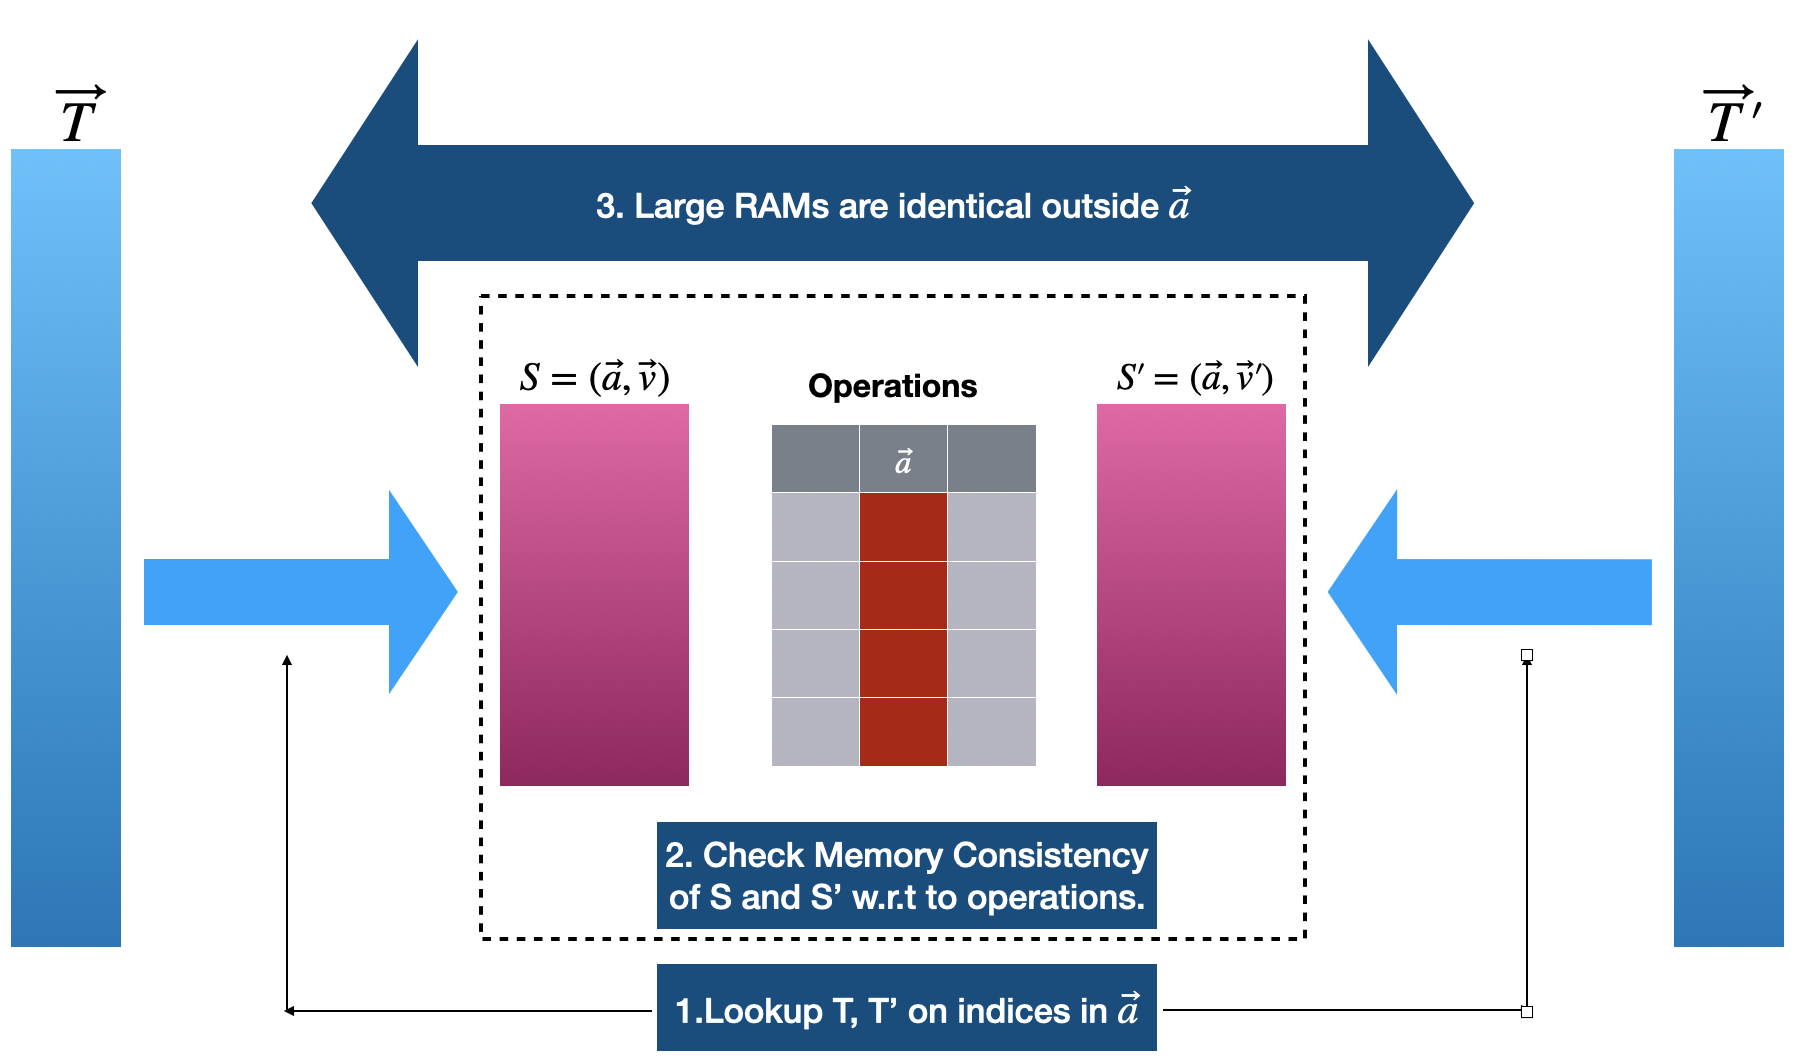
\includegraphics[width=0.4\textwidth]{RAM-Lookup}
    \caption{Illustrating different steps of sub-linear lookup protocol between large RAMs $\vecT$ and $\vecT'$.}
    \label{fig:blueprint}
\end{figure}

The blueprint for the above approach is illustrated in Figure ~\ref{fig:blueprint}.
The efficiency of the above approach relies crucially on the efficiency of committed index lookup used to
reduce the size of the RAMs for quasi-linear memory checking methods. It is tempting to use the recent lookup arguments
in ~\cite{CCS:ZBKMNS22,EPRINT:PosKat22,EPRINT:EagFioGab22} to prove the correctness of the first step with prover complexity dependent only on $m$.
However, employing them directly is difficult; their table-independent efficiency relies on
table specific expensive pre-computation, which does not help when the table is updatable. This is the problem we solve
in Section ~\ref{sec:update-protocol}, where we modify the prover algorithm for the lookup arguments to remain efficient
with access to pre-computed parameters for an ``approximate'' table.
\begin{comment} %repetition
In particular, we show that lookup protocols in
~\cite{CCS:ZBKMNS22,EPRINT:PosKat22,EPRINT:EagFioGab22} can be used to show $m$ lookups from a table $\vecT'$, given pre-computed parameters
for a table $\vecT$ with additional overhead of $O((m+\delta)\log^2 (m+\delta))$, where $\delta$ denotes the hamming distance
of tables $\vecT$ and $\vecT'$. By optimally deferring the $O(N\log N)$ re-computation till we
accumulate $\delta \approx \sqrt{mN}$ updates, we achieve an amortized prover overhead $O(\sqrt{mN})$ over the lookup protocols for non-updatable tables.
This modification described in ~\ref{sec:update-protocol} applies to all the aforementioned lookup protocols.
\end{comment}

\noindent{\bf Additional Notation}:
%Before proceeding, we introduce the subgroup $\setN=\{\xi,\ldots,\xi^N\}$ consisting of $N^{th}$ roots of unity,
%over which we encode vectors in $\F^N$ as polynomials of degree less than $N$. Let $\{\mu_i(X)\}_{i=1}^N$ be the associated
%lagrange basis polynomials over the set $\setN$. 
We introduce the set $\setV$ consisting of $m^{th}$ roots of unity
$\nu,\ldots,\nu^m$ with associated lagrange polynomials as $\{\tau_i(X)\}_{i=1}^m$. For $\vec{f}\in \F^N$, let
$\enc{f}{\setN}$ denote the polynomial encoding of $\vec{f}$ over $\setN$ given by $\sum_{i=1}^N f_i\mu_i(X)$. Similarly,
for $\vec{g}\in \F^m$, let $\enc{g}{\setV}$ denote its polynomial encoding over $\setV$ given by $\sum_{i=1}^m g_i\tau_i(X)$. 
For vectors $\vec{t}$, we sometimes use the index notation $\vec{t}[a_i]$ to denote $a_i^{th}$ element of the vector. For vectors
$\vec{t}$ and $\vec{a}$ we use the notation $\vec{t}[\,\vec{a}\,]$ to denote the vector $\vec{v}$ such that $v_i=\vec{t}[\,a_i\,]$ for all $i$.
%\chaya{above can be pruned. some of it is already in prelims.}


\subsection{Committed Index Lookup}\label{subsec:committed-index-lookup}
Let $m,N\in \N$ be fixed parameters with $m < N$ and let $\srs$ denote a $\kzg$ setup of degree $d\geq N$
over bi-linear group $(\F$, $\Gone$, $\Gtwo$, $\GT$, $e$, $\gone{1}$, $\gtwo{1}$, $[1]_t)$. Recall that the committed index
lookup relation in Definition ~\ref{defn:comm-index-lookup} involves the prover showing knowledge of vectors $\vecT\in \F^N$,
$\vec{a}\in \F^m$ and $\vec{v}\in \F^m$ corresponding to public commitments $c_T, c_a$ and $c_v$ such that they
satisfy $v_i = \vecT[\,a_i\,] = T_{a_i}$.
We present a polynomial protocol for the same, which is an adaptation of the lookup protocol from Caulk+ ~\cite{EPRINT:PosKat22}.
However, here we do not aim for zero-knowledge. Let $T(X)=\enc{t}{\setN}$, $a(X)=\enc{a}{\setV}$ and
$v(X)=\enc{v}{\setV}$ denote the polynomials encoding the vectors $\vec{t},\vec{a}$ and $\vec{v}$ respectively.
The verifier knows commitments to these polynomials at the start of the protocol.
Now $v_i = \vec{t}[a_i]$ for $i\in [m]$ is equivalent to $v(\nu^i) = T(\xi^{a(\nu^i)})$ for $i\in [m]$. To
obtain a polynomial protocol, the prover interpolates a polynomial $h(X)=\sum_{i=1}^m \xi^{a_i}\tau_i(X)$, which satisfies
$h(\nu^i)=\xi^{a(\nu^i)}$. To show that polynomial $h$ correctly ``exponentiates'' evaluations of $a(X)$, we consider the
inverting polynomial $\ell(X)=\sum_{i=1}^N i\mu_i(X)$ which behaves like ``log'' over $\setN$ by evaluating to $i$ on $\xi^i$. Now, we see
that all constraints are encoded as polynomial identities below:
\begin{equation}
    \begin{aligned}
        \ell(h(X)) &= a(X) \quad \text{mod } Z_{\setV}\\  % & \quad\text{ encodes } & \quad \forall i\in [m]:& h(\nu^i) = \xi^{a(\nu^i)}  \\
        T(h(X)) &= v(X) \quad \text{mod } Z_\setV \\ % \quad\text{ encodes } & \quad \forall i\in [m]:& v_i = \vec{t}[a_i] \\
        Z_{\setN}(h(X)) &= 0 \qquad \text{mod } Z_\setV  %&\quad\text{ encodes } & \quad \forall i \in [m]:& h(\nu^i)\in \setN
    \end{aligned}
    \label{eq:comm-index-lookup}
\end{equation}
The last polynomial identity ensures that evaluations of $h$ on $\setV$ lie in $\setN$ (the set of roots of $\vpolyN$). Since the polynomial $\ell$ is one-one
over $\setN$, the first equation implies $h(\nu^i)=\xi^{a_i}$ for all $i\in [m]$. The desired relation $v_i=T_{a_i}$ now follows from the second identity.
The above formulation involves composition with polynomials $\ell,T$ and $\vpolyN$ of degree $O(N)$, which is inefficient. We use the trick from
\cite{EPRINT:PosKat22}, where we work with low-degree restrictions of $O(N)$-degree polynomials such as $T, \ell$ over the set
$\setN_I=\{{h(\nu^i)}: i\in [m]\}=\{\xi^{a_i}:i\in I\}\subseteq \setN$, where $I=\{a_i: i\in [m]\}$. The prover
commits to the polynomials $Z_I(X)=\prod_{i\in I}(X-\xi^i)$, $h(X)$ and low degree ($<m$) restrictions $T_I, \ell_I$ of $T$ and $\ell$
on the $\setN_I$ respectively. The polynomial protocol then checks the following:
\begin{equation}
    \begin{alignedat}{3}
        T(X) - T_I(X) &= 0 \quad \text{ mod } Z_I ,&\quad& T_I(h(X)) &= v(X) \quad \text{ mod } Z_{\setV} \\
        \ell(X) - \ell_I(X) &= 0 \quad \text{ mod } Z_I ,&\quad& \ell_I(h(X)) &= a(X) \quad \text{ mod } Z_{\setV} \\
        Z_{\setN}(X) &= 0 \quad \text{ mod } Z_I ,&\quad& Z_I(h(X)) &= 0 \quad \text{ mod } Z_{\setV}
    \end{alignedat}
    \label{eq:poly-comm-index}
\end{equation}
It must be noted that the above identities imply the earlier polynomial identities in \eqref{eq:comm-index-lookup}. This is so because evaluations
of $h$ on $\setV$ are roots of $Z_I$, which implies $T_I(h(\nu^i))=T(h(\nu^i))$, $\ell_I(h(\nu^i))=\ell(h(\nu^i))$ and $\vpolyN(h(\nu^i))=0$ over $\setV$.
While the identities on the left still involve a degree $N$ polynomial, we can use the $\srs$ to check the polynomial
identity at the point $\tau$ encoded in the $\srs$. For example, we can evaluate the encoded quotient $\gtwo{Q(X)} =$
$\gtwo{\frac{(T(X) - T_I(X)}{Z_I(X)}}$ using the relation:
\begin{equation*}
    \gtwo{\frac{T(X)-T_I(X)}{Z_I(X)}} = \sum_{i\in I}\frac{1}{Z_I'(\xi^i)}\gtwo{\frac{T(X)-t_i}{X-\xi^i}}
\end{equation*}
By pre-computing the $\kzg$ proofs $W_1^i=\gtwo{\frac{T(X)-t_i}{X-\xi^i}}$ for all $i\in [N]$, the encoded quotient can be
evaluated using $O(m)$ $\Gtwo$-operations and $O(m\log^2 m)$ $\F$-operations.
The identity is then checked using a real pairing check
$$e(\gone{T(X)}-\gone{T_I(X)},\gtwo{1})=e(\gone{Z_I(X)},\gtwo{Q(X)}).$$
Similarly, we also pre-compute the encoded
quotients $W_2^i=\gtwo{\frac{\ell(X) - i}{X-\xi^i}}$ and $W_3^i=\gtwo{\frac{\vpolyN(X)}{X-\xi^i}}$ for all $i\in [N]$.
The quotients can be computed in time $O(N\log N)$ using the techniques in ~\cite{EPRINT:FeiKho23}. Using $\kzg$ commitment
scheme the polynomial relations over $Z_\setV$ can be checked in a standard manner
by having the prover send evaluation proofs for the committed polynomials at a random point chosen by the verifier.
The total prover effort incurred is $O(m^2)$ group and field operations.
Thus, we have:
\begin{lemma}\label{lem:comm-index-lookup}
Assuming $\kzg$ is extractable polynomial commitment scheme, there exists a succinct argument of knowledge for
the relation $\RLOOK$ with prover complexity of $O(m^2)$, given access to pre-computed parameters of size $O(N)$.
\end{lemma}

\subsubsection{Committed Index Lookup: Generic Transformation}\label{subsubsec:generic-transformation}
The protocol for committed index lookup using Caulk+ ~\cite{EPRINT:PosKat22} can become prohibitive for higher values of
$m$ due to the quadratic dependence on it. Here we describe a generic transformation, which realizes a committed index lookup
argument from any sub-vector argument such as ~\cite{CCS:ZBKMNS22,EPRINT:PosKat22,EPRINT:ZGKMR22,EPRINT:EagFioGab22} using a homo-morphic
vector commitment scheme. We recall that $\vec{a}\in \F^m$ is called a sub-vector of $\vec{b}\in \F^n$ if each element of $\vec{a}$
also occurs in $\vec{b}$. We use $\vec{a}\leq \vec{b}$ to denote $\vec{a}$ is a sub-vector of $\vec{b}$.
The transformation follows from the observation in the following lemma:
\begin{lemma}\label{lem:generic-transformation}
Let $\vec{t}\in \F^n$ and let $\vec{a},\vec{v}\in \F^m$ for some positive integers $m,n$. Let $\vec{I}_n$ denote the vector $(1,\ldots,n)$.
Then for $\gamma\gets \F$, $\vec{a}\leq \vec{I}_n$, $\vec{v}\leq \vec{t}$ and $(\vec{v}+\gamma \vec{a})\leq (\vec{t} + \gamma \vec{I}_n)$ implies
$\vec{v}=\vec{t}[\,\vec{a}\,]$ except with probability $O(n/|\F|)$.
\end{lemma}
The proof of the Lemma appears in Section ~\ref{sec:generic-transformation-app}.
Using Lemma ~\ref{lem:generic-transformation}, allows construction of argument for proving $\vec{v}=\vec{t}[\,\vec{a}\,]$ using three instantiations
of a sub-vector argument. We require homomorphism of the commitment scheme to enable the verifier to compute commitments for $\vec{v}+\gamma \vec{a}$ and
$\vec{t} + \gamma \vec{I}_n$ for the final instantiation of sub-vector argument. In particular, we also benchmark committed index lookup
protocol using lookup argument in ~\cite{EPRINT:EagFioGab22}, which incurs prover complexity of $O(m\log m)$.
~

\subsection{Almost Identical RAM States}\label{subsec:proximity-ram}
For a vector $\vec{a}\in [N]^m$, let $\uniq{a}=\{a_i: i\in [m]\}$ denote the subset of unique values in $\vec{a}$. We call two
RAM states $\vecT, \vecT'\in \F^N$ to be $\vec{a}$-{\em identical} if $\vecT[i]=\vecT'[i]$ for all $i\not\in\uniq{a}$. As before,
let $T(X),T'(X)$ and $a(X)$ be polynomials encoding the vectors $\vecT,\vecT'$ (over $\setN$) and $\vec{a}$ (over $\setV$). Given
commitments $c_T, c_T'$ and $c_a$ polynomial protocol to prove that committed vectors $\vecT,\vecT'\in \F^N$ and $\vec{a}\in \F^m$
are such that $\vecT,\vecT'$ are $\vec{a}$-identical involves proving the relation $Z_I(X)(T(X) - T'(X)) = 0$ over $Z_\setN$ where
$I=\uniq{a}$ and $Z_I(X)=\prod_{i\in I}(X-\xi^i)$ denotes the vanishing polynomial for the set $\setN_I=\{\xi^i: i\in I\}$.
The prover commits to polynomial $Z_I$ and proves (i) $Z_I(T - T') = 0 \text{ mod } Z_\setN$ and (ii) $Z_I$ is the vanishing
polynomial of the set $\setN_I$ as defined. To prove the first relation, the prover computes the polynomial $Q(X)$ as below:
\begin{align}\label{eq:poly-q}
D(X) &= \frac{(T(X)-T'(X))\cdot Z_I(X)}{Z_\setN(X)} \nonumber \\
&= \sum_{i\in I}\frac{(t_i - t_i')\mu_i(X)}{Z_\setN(X)} Z_I(X) \nonumber \\
\intertext{ Substituting, $\Delta_i=t_i-t_i'$, $\mu_i(X)=\vpolyN(X)/(\vpolyN'(\xi^i)(X-\xi^i))$ }
&=\sum_{i\in I}\frac{\Delta_i}{Z_\setN'(\xi^i)}\left(\frac{Z_I(X)}{X-\xi^i}\right) = \sum_{i\in I}\frac{\Delta_i Z_I'(\xi^i)}{Z_\setN'(\xi^i)}\kappa_i(X)
\end{align}
In the above, the summation only runs over indices in $I$, as $\Delta i = 0$ for $i\not\in I$. In the final equality, we use
$\kappa_i(X) = Z_I(X)/(Z_I'(\xi^i)(X-\xi^i))$ for $i\in I$ which we recognize as the lagrange basis polynomials for the set
$\{\xi^i: i\in I\}$. Thus, Equation \eqref{eq:poly-q} implies that $D(X)$ is at most degree $|I|-1$ polynomial, with
$D(\xi^i)=\Delta_i Z_I'(\xi^i)/\vpolyN'(\xi^i)$ for $i\in I$.
The prover can therefore interpolate $D(X)$ (in power basis)
in $O(|I|\log^2 |I|)$ $\F$-operations and compute $\gone{D(X)}$ in $O(|I|)$ $\Gone$-operations. The prover sends the
commitment $\gone{D(X)}$ to the verifier. Finally, the verifier can
check the identity $Z_I(T - T') = D\cdot Z_\setN$ by a pairing check. For this, since the tables are committed in $\Gone$, prover will need to send $\elttwo{Z_I(X)}$.

Next, the prover needs to show that $Z_I(X)$ is indeed the vanishing polynomial of $\setN_I$.
We again use the polynomial $h(X)=\sum_{i=1}^m \xi^{a_i}\tau_i(X)$ which interpolates the vector $(\xi^{a_1},\ldots,\xi^{a_m})$.
The correctness of the $h$ polynomial can be established by checking the polynomial identities in the last two rows of Equation
~\eqref{eq:poly-comm-index}. The aforementioned identities show that $Z_I(h(X)) = 0$ over $Z_\setV$ which shows that $Z_I$ vanishes over
entire vector interpolated by $h$ over $\setV$. To assert that $Z_I$ has no additional roots, the prover commits to the product polynomial
$K(X)=\prod_{i=1}^m (X - h(\nu^i))$ and the quotient polynomial $q(X)=K(X)/Z_I(X)$. The verifier checks the polynomial identities
at $\alpha$, i.e $K(\alpha)=q(\alpha)Z_I(\alpha)$ and $K(\alpha)=\prod_{i=1}^m(\alpha - h(\nu^i))$.
The former is easily accomplished
using evaluation proofs for $K,q$ and $Z_I$ at $\alpha$
For checking the latter, the prover commits to another polynomial
$u(X)$ satisfying $u(\nu^i)=\prod_{j=1}^{i-1}\big((\alpha - h(\nu^j))/(1 + \beta\tau_1(\nu^j))\big)$ for $i\in [m]$
where $\beta=K(\alpha) - 1$.
The verifier ensures the correctness of $u(X)$ by
\begin{equation}
    \begin{aligned}
        \tau_1(X)(u(X) - 1) &= 0 \text{ mod } Z_{\setV} \\
        u(\nu X)(1+\beta \tau_1(X))-u(X)(\alpha - h(X)) &= 0 \text{ mod } Z_\setV.
    \end{aligned}
    \label{eq:kh-check}
\end{equation}
We prove that the above constraints imply that $K(\alpha)=\prod_{i\in [m]}(\alpha - h(\nu^i))$.
Note that in this protocol we require commitment to the polynomial $Z_I$ in both $\Gone$ and $\Gtwo$,
and thus another pairing check is required to show that the $Z_I(X)$ committed in $\Gone$
(whose well formation is shown in the protocol as described above) is the same as the $Z_I(X)$ committed in $\Gtwo$,
used for the real pairing check.
\begin{lemma}\label{lem:kh-check}
There exists a polynomial $u(X)\in \F[X]$ satisfying the identities in Equation ~\eqref{eq:kh-check}
if and only if $K(\alpha)=1+\beta=\prod_{i\in [m]} (\alpha - h(\nu^i))$.
\end{lemma}
\begin{proof}
    Assume that the identitites hold for some polynomial $u(X)$.
    The first identity implies $u(\nu)=1$. From the second identity, we conclude that for all $i\in [m]$, we have
    $u(\nu^{i+1})=u(\nu^i)\cdot ((\alpha - h(\nu^i))/(1+\beta \tau_1(\nu^i)))$, and thus:
    $$1 = u(\nu^{m+1})/u(\nu) = \prod_{i\in [m]}\left(\frac{\alpha - h(\nu^i)}{1+\beta \tau_1(\nu^i)}\right).$$
    We observe that the product of denominators in the above equation is simply $1+\beta$ as $\tau_1(\nu^i)$
    is $0$ for all $i\neq 1$, and thus $1+\beta = \prod_{i=1}^m (\alpha - h(\nu^i))$. In the other direction,
    it is easy to check that $u(X)$ as defined for an honest prover, satisfies the identities in Equation ~\ref{eq:kh-check}.
\end{proof}

\noindent{\em Remark}: Note that we incur $O(m^2)$ cost if we show the correctness of polynomial $h$ using techniques of Section ~\ref{subsec:committed-index-lookup}.
However, we can use more $O(m\log m)$ complexity committed index lookup obtained from ~\cite{EPRINT:EagFioGab22}, which allows us to show correctness of
$h(X)$ by proving that it interpolates vector $\vec{h}$ on $\setV$ obtained as committed index lookup using vector $\vec{a}$ on the vector $\vecT_{exp}=(\xi,\xi^2,\ldots,\xi^N)$
i.e., $\vec{h}=\vecT_{exp}[\, \vec{a}\,]$.

\subsection{Batching Efficient RAM: Combined Protocol}\label{subsec:all-together}
We put the entire protocol together now. Let $\setind$ denote the set of indices $\{1,\ldots,N\}$, and $\mathcal{I}_N$
denote the vector $(1,\ldots,N)$. We formally define the committed RAM relation for which we present an argument of
knowledge in this section.
\begin{definition}\label{defn:committed-ram}
We define the {\em committed ram} relation
$\CRAM$ to consist of tuples $((c_T, c_T', c_\op, c_a, c_w),(\vecT, \vecT',\vec{\op},\vec{a},\vec{w}))$
such that:
\begin{itemize}[leftmargin=1em]
    \item $(T,\vec{o},T')\in \LRAM{I}{N}{m}$ for $T=(\setind_N,\vecT)$, $T'=(\setind_N,\vecT')$ and $\vec{o}=(o_1,\ldots,o_m)$
    where $o_i=(\op_i, a_i, w_i)\in \RAMOp{I}$ for all $i\in [m]$.
    \item $c_T=\KZGcommit(\srs, T(X))$, $c_T'=\KZGcommit(\srs, T'(X))$, $c_\op = \KZGcommit(\srs,\op(X))$,  $c_a=\KZGcommit(\srs, a(X))$,
    $c_w = \KZGcommit(\srs, w(X))$ where polynomials $T(X), T'(X)$ encode vectors $\vecT, \vecT'$ over $\setN$, while $\op(X), a(X)$ and
    $w(X)$ encode vectors $\vec{\op}=(\op_1,\ldots,\op_m)$, $\vec{a}$ and $\vec{w}$ over $\setV$.
\end{itemize}
\end{definition}
As outlined in the blueprint, the prover first commits to ``smaller'' RAMs $S=(\vec{a},\vec{v})$ and $S'=(\vec{a},\vec{v}')$
where $\vec{v}=\vecT[\vec{a}]$ and $\vec{v}'=\vecT'[\vec{a}]$. The prover commits to $S$ and $S'$ by sending commitments
$c_v$ and $c_v'$ to $\vec{v}$ and $\vec{v}'$. Then the prover and verifier execute the committed index lookup protocol to
prove:
\begin{equation}
(c_T, c_a, c_v)\in \RLOOK\, \wedge\, (c_T', c_a, c_v')\in \RLOOK
\end{equation}
The verifier uses a random challenge $\chi\gets \F$ to reduce two instances of $\RLOOK$ to one instance
$(c_T + \chi c_T', c_a, c_v + \chi c_v')\in \RLOOK$. Then, we show that
RAMs $\vecT$ and $\vecT'$ are $\vec{a}$-identical using the protocol in Section \ref{subsec:proximity-ram}.
All that remains is to prove is that the operation sequence $\vec{o}$ is consistent with small RAMs $S$ and $S'$.
We check this using the argument in Section ~\ref{sec:poly-proto-ram}. Specifically, the prover and the verifier set
$c_S = (c_a, c_v)$, $c_S'=(c_a, c_v')$ and $c_o = (c_\op, c_a, c_w)$, and execute the argument of knowledge for
showing $(c_S, c_o, c_S')\in \CLRAM$ (see Definition ~\ref{defn:committed-ram}). We provide the complete protocol
listing in Figure ~\ref{fig:complete-listing}. The protocol in Figure ~\ref{fig:complete-listing} assumes pre-computed parameters
for the tables $T$ and $T'$. In the next section, we discuss how to efficiently maintain table-dependent parameters in the setting
requiring updates to the table.

\begin{theorem}\label{thm:committed-ram}
The protocol in Figure~\ref{fig:complete-listing} (continued in Figures~\ref{fig:complete-listing-2} and
~\ref{fig:complete-listing-3}) is a succinct argument of knowledge for the relation $\CLRAM$ in
the AGM, under the $Q$-DLOG assumption for the bilinear group $(\F,\Gone,\Gtwo,\GT,e,g_1,g_2)$.
\end{theorem}

%%% complete protocol listing %%%
\begin{figure}[t!]
    \begin{mdframed}

        \underline{Setup $(1^\secp,N,m, \vecT, \vecT')$}:
        \begin{itemize}[leftmargin=1em]
            \item $\srs = (\{\gone{\tau^i}\}_{i=0}^N, \{\gtwo{\tau^i}\}_{i=0}^N)$ for $\tau\gets \F$.
            \item $W_2^i=\gtwo{(\ell(X) - i)/(X-\xi^i)}$, $i\in [N]$(needed by prover)
            \item $W_3^i=\gtwo{\vpolyN(X)/(X-\xi^i)}$, $i\in [N]$(needed by prover)
            \item $\gone{\ell(X)}, \gone{\vpolyN(X)}, \gtwo{\vpolyN(X)}$(known by both)
        \end{itemize}

        \underline{Precompute $(\vecT, \vecT')$}:
        \begin{itemize}[leftmargin=1em]
            \item $W_1^i=\gtwo{(T(X)-T(\xi^i))/(X-\xi^i)}$, $i\in [N]$,
            \item ${W_1^i}'=\gtwo{(T'(X) - T'(\xi^i))/(X-\xi^i)}$, $i\in [N]$.
        \end{itemize}

        {\bf Common Input}: $\srs$, $c_T, c_T', c_\op, c_a, c_w\in \Gone$.\\
        {\bf Prover's Input}: Vectors $\vecT,\vecT',\vec{\op},\vec{a},\vec{w}$ and their encoding polynomials.\\

        {\bf Round 1}: Commit to sub RAMs.
        \begin{enumerate}[leftmargin=1em, label=\arabic*.]
            \item $\prover$ computes $\vec{v}=\vecT[\,\vec{a}\,]$, $\vec{v}'=\vecT'[\,\vec{a}\,]$ and the encoding
            polynomials $v(X)$ and $v'(X)$.
            \item $\prover$ sends $c_v = \gone{v(X)}$, $c_v'=\gone{v'(X)}$.
            \item $\verifier$ sends $\chi\gets \F$.
        \end{enumerate}

        {\bf Round 2}: Execute committed index lookup.
        \begin{enumerate}[leftmargin=1em, label=\arabic*.]
            \item $\prover$ and $\verifier$ compute $C_T=c_T + \chi c_T'$, $C_V=c_v + \chi c_v'$.
            \item $\prover$ computes $P(X) = T(X) + \chi T'(X)$, $V(X)=v(X) + \chi v'(X)$.
            \item $\prover$ computes $I=\{a_i: i\in [m]\}$, $\setN_I=\{\xi^i: i\in I\}$.
            \item $\prover$ computes polynomials:
            \begin{itemize}[leftmargin=1em, label=-]
                \item Vanishing polynomial $Z_I(X)$ of $\setN_I$.
                \item Polynomial $h(X)=\sum_{i\in [m]}\xi^{a_i}\tau_i(X)$.
                \item Restrictions $P_I(X),\ell_I(X)$ of $P(X),\ell(X)$ on set $I$.
                \item $K(X)=\prod_{i\in [m]}(X-\xi^{a_i})$, $q(X)=K(X)/Z_I(X)$
                \item $D(X)= \sum_{i\in I}\frac{\Delta_i Z_I'(\xi^i)}{Z_\setN'(\xi^i)}\kappa_i(X)$ by interpolation as described in section 5.2
            \end{itemize}

            \item $\prover$ sends $c_p = \gone{P_I(X)}$, $c_z=\gone{Z_I(X)}$, $c_{z2}=\gtwo{Z_I(X)}$, $c_h=\gone{h(X)}$, $c_l = \gone{\ell_I(X)}$,
            $c_k = \gone{K(X)}$, $c_q = \gone{q(X)}$, $c_d=\gone{D(X)}$
            \item $\verifier$ sends $\gamma\gets \F$.
        \end{enumerate}

        {\bf Round 3}: Prover send aggregated quotients.
        \begin{enumerate}[leftmargin=1em, label=\arabic*.]
            \item $\prover$ computes $g(X)=P_I(X) + \gamma \ell_I(X) + \gamma^2 Z_I(X)$.
            \item $\prover$ computes $Q(X) = (g(h(X)) - v(X) -\gamma a(X))/Z_\setV(X)$.
            \item $\prover$ computes: $W = \sum_{i\in [m]} \frac{1}{Z_I'(\xi^i)} (W_1^i + \chi {W_1^i}' + \gamma W_2^i + \gamma^2 W_3^i)$.
            \item $\prover$ sends $W\in \Gtwo$, $c_Q=\gone{Q(X)}$.
            \item $\verifier$ computes $c_g = c_p + \gamma c_l + \gamma^2 c_z$, $C_G = C_T + \gamma\gone{\ell(X)}+\gamma^2\gone{\vpolyN(X)}$.
            \item $\verifier$ checks: $e(C_G - c_g, \gtwo{1})=e(c_z, W)$.
            \item $\verifier$ checks: $e(c_T-c_{T'}, c_{z2})=e(c_d, \gtwo{\vpolyN(X)})$
            \item $\verifier$ checks: $e(c_z, [1]_2)=e([1]_1, c_{z2})$
            \item $\verifier$ sends $\alpha\gets \F$.
        \end{enumerate}

        Continued in Figure ~\ref{fig:complete-listing-2}
    \end{mdframed}
    \caption{Batching Efficient RAM Protocol}
    \label{fig:complete-listing}
\end{figure}

\begin{figure}[t!]
    \begin{mdframed}
        \begin{center}
            Continued from Figure \ref{fig:complete-listing}
        \end{center}
        {\bf Round 4}: Prover sends evaluations.
        \begin{enumerate}[leftmargin=1em, label=\arabic*.]
            \item $\prover$ computes $\val{\alpha}{v}=v(\alpha)$, $\val{\alpha}{a}=a(\alpha)$, $\val{\alpha}{h}=h(\alpha)$, $\val{\alpha}{K}=K(\alpha)$,
            $\val{h(\alpha)}{g}=g(h(\alpha))$, $\val{\alpha}{Q}=Q(\alpha)$, $\val{\alpha}{q}=q(\alpha)$, $\val{\alpha}{Z}=Z_I(\alpha)$.
            \item $\prover$ sends $\val{\alpha}{v}$, $\val{\alpha}{a}$, $\val{\alpha}{h}$, $\val{\alpha}{K}$, $\val{h(\alpha)}{g}$, $\val{\alpha}{Q}$,
            $\val{\alpha}{q}$, $\val{\alpha}{Z}$
            \item $\prover$ computes polynomial $u(X)$ as in Section ~\ref{subsec:proximity-ram}
            and sends $c_u=\gone{u(X)}$.
            \item $\verifier$ checks $\val{\alpha}{Q}(\alpha^m-1)=\val{h(\alpha)}{g}-\val{\alpha}{v}-\gamma \val{\alpha}{a}$.
            \item $\verifier$ checks $\val{\alpha}{Z}\val{\alpha}{q}=\val{\alpha}{K}$.
            \item $\verifier$ sets $\beta=\val{\alpha}{K}-1$ and sends $\theta\gets\F$.
        \end{enumerate}

        {\bf Round 5}: Check correctness of $K$.
        \begin{enumerate}[leftmargin=1em, label=\arabic*.]
            \item $\prover$ computes:
            \begin{align*}
                Q'(X) &= \big(u(\nu X)(1+\beta \tau_1(X))-u(X)(\alpha - h(X)) \\
                &\quad + \theta \tau_1(X)(u(X)-1)\big)/Z_\setV(X).
            \end{align*}
            \item $\prover$ sends $c_Q'=\gone{Q'(X)}$.
            \item $\verifier$ sends $x\gets \F$.
        \end{enumerate}

        {\bf Round 6}: Prover sends more evaluations.
        \begin{enumerate}[leftmargin=1em, label=\arabic*.]
            \item $\prover$ computes $\val{x}{u}=u(x)$, $\val{\nu x}{u}=u(\nu x)$, $\val{x}{h}=h(x)$, $\val{x}{Q'}=Q'(x)$
            \item $\prover$ sends $\val{x}{u}$, $\val{\nu x}{u}$, $\val{x}{h}$, $\val{x}{Q'}$.
            \item $\verifier$ checks $\val{x}{Q'}(x^m-1)=\val{\nu x}{u}(1+\beta \tau_1(x))-\val{x}{u}(\alpha - \val{x}{h})$.
            \item $\verifier$ sends $r_a, r_h, r_q, r_v, r_K, r_Q, r_Z\gets \F$ and $r_h', r_u', r_Q'\gets \F$.
        \end{enumerate}

        \begin{center}
        Continue in Figure ~\ref{fig:complete-listing-3}.
        \end{center}


    \end{mdframed}
    \caption{Batching Efficient RAM Protocol: Continued}
    \label{fig:complete-listing-2}
\end{figure}

\begin{figure}[t!]
    \begin{mdframed}
        \begin{center}
            Continued from Figure \ref{fig:complete-listing-2}
        \end{center}
        \item {\bf Round 7}: Check aggregated evaluation.
        \begin{enumerate}[leftmargin=1em, label=\arabic*.]
            \item $\prover$ computes:
            \begin{align*}
                \Phi_\alpha(X) &= r_a a(X)+ r_h h(X) + r_q q(X) + r_v v(X) \\
                &\quad + r_K K(X) + r_Q Q(X) + r_Z Z_I(X) \\
                \Phi_x(X) &= r_h' h(X) + r_u' u(X)+r_Q'Q'(X)
            \end{align*}
            \item $\prover$ computes $\Pi_\alpha = \KZGopen(\srs, \Phi_\alpha(X), \alpha)$.
            \item $\prover$ computes $\Pi_x = \KZGopen(\srs, \Phi_x(X), x)$.
            \item $\prover$ computes $\Pi_g = \KZGopen(\srs, g(X), \val{\alpha}{h})$.
            \item $\prover$ computes $\Pi_u = \KZGopen(\srs, u(X), \nu x)$.
            \item $\prover$ sends $\Pi_\alpha$, $\Pi_x$, $\Pi_g$ and $\Pi_u$.
            \item $\verifier$ computes:
            \begin{align*}
                \gone{\Phi_\alpha} &= r_a c_a + r_h c_h + r_q c_q + r_v c_v + r_z c_z + r_K c_K + r_Q c_Q. \\
                \gone{\Phi_x} &= r_h' c_h + r_u' c_u + r_Q' c_Q' \\
                V_{\alpha} &= r_a \val{\alpha}{a} + r_h \val{\alpha}{h} + r_q \val{\alpha}{q} + r_v \val{\alpha}{v} \\
                &\quad + r_z\val{\alpha}{Z} r_K \val{\alpha}{K} + r_Q \val{\alpha}{Q}. \\
                V_x &= r_h' \val{x}{h} + r_u' \val{x}{u}+r_Q' \val{x}{Q'}
            \end{align*}
            \item $\verifier$ checks:
            \begin{itemize}[leftmargin=1em]
                \item $\KZGverify(\srs, \gone{\Phi_\alpha}, V_\alpha, \alpha, \Pi_\alpha)$.
                \item $\KZGverify(\srs, \gone{\Phi_x}, V_x, x, \Pi_x)$.
                \item $\KZGverify(\srs, c_g, \val{h(\alpha)}{g}, \val{\alpha}{h}, \Pi_g)$.
                \item $\KZGverify(\srs, c_u,\val{\nu x}{u}, \nu x, \Pi_u)$.
            \end{itemize}
            \item $\prover$ and $\verifier$ set $c_S=(c_a, c_v)$, $c_S'=(c_a, c_v')$, $c_o=(c_\op, c_a, c_w)$.
            \item $\prover$ and $\verifier$ execute argument for $(c_S, c_o, c_S')\in \CLRAM$ (Section ~\ref{sec:poly-proto-ram}).
        \end{enumerate}
    \end{mdframed}
    \caption{Batching efficient RAM Protocol-Continued}
    \label{fig:complete-listing-3}
\end{figure}





\section{Fast Lookups from Approximate Pre-Processing}\label{sec:update-protocol}


Recall that our lookup protocol in section 5.1 involves certain precomputations by the prover namely $W_1^i, W_2^i, W_3^i$. $W_2^i$ and $W_3^i$ do not depend on the table. However, $W_1^i$ depends on the lookup table and their values will change even if the table changes by a small amount. It is expensive to recompute all the $W_1^i$ for every small change in the table and this will affect the efficiency of our lookup protocol in the long run.\\\\
In this section, we show how to achieve efficient lookups even when the table is changing frequently, as long as the cumulative change in the table is small. \\
In particular, we show how the prover can compute $[Q(X)]_2=\gtwo{\frac{T(X)-T_I(X)}{Z_I(X)}}$ without computing all the $W_1^i$(thus minimizing the overhead).\\
The overhead(as long as the table doesn't change too much) will be much lower than the time needed for the lookup and so is very practical.

\subsection{The idea: Base + Cache approach}

The idea is that we do not compute $W_1^i$ after each change of the table. Instead, this expensive computation will be done periodically for all $i \in [N]$ after say $s \in \mathbb{Z}$ batches.
Let current table $\vecT$ can be represented as $\vecTbase + \vecTcache$ where the vector
$\vecTbase$ denotes the base table (with respect to which $W_1^i$ was last computed for all $i \in [N]$) and the vector $\vecTcache$ corresponds to the changes
that have happened to the base table since the last rebasing (rebasing denotes computation of all $W_1^i$)\\\\
Thus, there is an \textbf{online} phase which happens after every batch (which includes computation of $[Q(X)]_2$ among other things) and an \textbf{offline} phase which consists of the rebasing(this is all prover computations) \\\\




\noindent{\bf Offline Phase}: This computation is executed once after every $s$ rounds. Here, the prover updates the base vector $\vecTbase$ with the changes in the cache vector
$\vecTcache$ by setting $\vecTbase := \vecTbase + \vecTcache$ and simultaneously clears the cache vector by setting
$\vecTcache = 0$.\\
It computes the commitment of $T_b$ as well\\
It also re-computes the $\mathsf{KZG}$ opening proofs $[W_1^i(x)]_2$ for $i\in [N]$ where
$W_1^i(X) = (\Tbasepoly{X} - t_i)/(X-\xi^i)$. Here, $t_i=\Tbasepoly{\xi^i}$ are the coordinates
of the updated base vector $\vecTbase$.\\
As mentioned in section 5.1 this can be done in $O(N\log N)$ group and field operations.\\\\
\noindent{\bf Online Phase}:
The online phase happens for every batch because the purpose of this phase is to ensure that all the things needed for the current execution of the lookup protocol are available. We show how the prover computes the next table $T'$ from the current table $T$ and the new Cache vector from the old cache vector (by an inductive argument this suffices)
\begin{enumerate}[leftmargin=1em]
    \item Prover has the $T$ for the current round and the commitment $[T(x)]_1$ as well(because these are just the $T'$, $[T'(x)]_1$ of the last round)
    \item The $\vecTcache$ and $\vecTcache(X)$ is also updated to the start of the current round (contains information till previous round:$\vecT=\vecTbase+\vecTcache$)
    \item The prover updates the cache using the current batch: $\vec{T'}_{\mathsf{ch}}[i] = \vec{T}_{\mathsf{ch}}[i] + \Delta_i$ for $i\in I$ in $O(m)$ $\F$ operations
    \item Here $\Delta_i$ for all $i \in I$ is the change that will happen to $\vecT$ \textbf{during the current round}
    \item Prover computes the commitment to the new cache polynomial:
    $$[\vec{T'}_{\mathsf{ch}}(x)]_1=[\vec{T}_{\mathsf{ch}}(x)]_1+\sum_{i\in I}\Delta_i[\mu_i(x)]_1$$ in
    $O(m)$ $\Gone$ operations.
    \item Prover also gets ${T}'$ as ${T'}[i]=T_b[i]+ \vec{T'_{\text{ch}}}[i]$ using the $T_b$ and the latest cache
    \item Prover computes the commitment to the new table $\vecT'$: $[T'(x)]_1=[\Tbasepoly{x}]_1+[\vec{T'}_{\mathsf{ch}}(x)]_2$

    \item In addition, the other things (apart from $[Q(x)]_2$) needed for the current round of the lookup protocol are also computed by the prover as described in the lookup protocol in section 5.1 as it is just naive computation



\end{enumerate}

\subsection{Computation of $[Q(X)]_2$}
Clearly, it suffices to efficiently compute $[Q(x)]_2$ where $[Q(x)]_2=\gtwo{\frac{T(x)-T_I(x)}{Z_I(x)}}$. We have the information of $[\Tbasepoly{x}-\Tbasepoly{\xi^i}/(x-\xi^i)]_2$. For this, we have the following lemma:


\begin{lemma}\label{lem:approx-setup}
Let $N,\xi$ be as defined previously. Suppose we are given
$\kzg$ proofs $\{W_i\}_{i=1}^N$ with $W_i=\gtwo{\Tbasepoly{X} - \Tbasepoly{\xi^i}/(X-\xi^i)}$ and where
$\Tbasepoly{X}=\enc{T_{\mathsf{b}}}{\setN}$ encodes a vector $\vecTbase\in \F^N$.
Let $I \subset [N]$.
Then,
there exists an algorithm to compute $\kzg$ multi-opening proof
$[Q(X)]_2=\gtwo{(T(x) - T_I(x)/Z_I(x)}$ for encoding $T(X)=\enc{T}{\setN}$ of vector $\vecT\in \F^N$ using $O((\delta + |I|) \log^2 (\delta + |I|))$ $\F$-operations and $O(\delta + |I|)$ $\Gtwo$-operations.
Here, $\delta$ denotes the hamming distance
between vectors $\vecTbase$ and $\vecT$.
\end{lemma}

\begin{proof}
    We know that $\vecT=\vecTbase+\vecTcache$ and that $T(X)=\Tbasepoly{X}+\Tcachepoly{X}$\\

    Let $K \subset [N]$ be a set which contains $I$ and all those indices $j$ for which $\vecTcache[j] \neq 0$. For these $j$, let $\vecTcache[j]=\Delta t_j$. Then $\Tcachepoly{X}=\sum_{j\in K}\Delta t_j\mu_j(X)$.\\\\
    By definition of $K$, $|K|\leq \delta +|I|$. So, we need to bound $\Gtwo$ operations by $O(|K|)$ and field operations by $O(|K| \log^2|K|)$\\
    First of all note that:
    \begin{align}\label{eq:Q2-upd}
    Q_2(X) &= \sum_{i\in \setind}\frac{1}{z_I'(\xi^i)}\left(\frac{\Tbasepoly{X} - \Tbasepoly{\xi^i}}{X-\xi^i}\right)
    + \sum_{i\in \setind}\frac{1}{z_I'(\xi^i)}\left(\frac{\Tcachepoly{X} - \Tcachepoly{\xi^i}}{X-\xi^i}\right)
    \end{align}

    From the above we can write $\elttwo{Q_2(x)}=\gtwo{\Qbasepoly{x}}+\gtwo{\Qcachepoly{x}}$ where
    \begin{gather*}
        \Qbasepoly{X}=\sum_{i\in \setind}(z_I'(\xi^i))^{-1} (\Tbasepoly{X}-\Tbasepoly{\xi^i})/(X-\xi^i) \\
        \Qcachepoly{X}=\sum_{i\in \setind}(z_I'(\xi^i))^{-1} (\Tcachepoly{X}-\Tcachepoly{\xi^i})/(X-\xi^i)
    \end{gather*}
    We can compute
    $\elttwo{\Qbasepoly{x}}$ from the pre-computed KZG openings of $\Tbasepoly(X)$ at points $\xi^i,i\in I$ using $O(|I|)$ group operations and
    $O(|I|\log^2 |I|)$ field operations(as is done in Caulk/Caulk+).\\\\

    \textbf{Thus, it suffices to describe the computation for $\elttwo{\Qcachepoly{x}}$. }\\
    Using
    $\Tcachepoly{X}=\sum_{j\in K}\Delta t_j\mu_j(X)$ and defining constants $c_i=(1/z_I'(\xi^i))$ for $i\in I$,
    we write $\Qcachepoly{X}$ as:
    \begin{align*}
        \Qcachepoly{X} &= \sum_{i\in \setind} c_i\sum_{j\in K} \Delta t_j\frac{\mu_j(X)-\mu_j(\xi^i)}{X-\xi^i} \\
        &= \sum_{i\in \setind} c_i\Delta t_i\frac{\mu_i(X) - 1}{X-\xi^i} + \sum_{i\in \setind}\sum_{j\in K\setminus\{i\}}c_i\Delta t_j\frac{\mu_j(X)}{X-\xi^i}
    \end{align*}
    Now, we can write $\elttwo{\Qcachepoly{x}}=\elttwo{\Qcachepolyone{x}} + \elttwo{\Qcachepolytwo{x}}$ where:
    \begin{gather*}
        \Qcachepolyone{X}=\sum_{i\in \setind}c_i\Delta t_i\frac{\mu_i(X)-1}{X-\xi^i} \\
        \Qcachepolytwo{X}=\sum_{i\in \setind}\sum_{j\in K\setminus \{i\}} c_i\Delta t_j\frac{\mu_j(X)}{X-\xi^i}
    \end{gather*}

    The term $\elttwo{\Qcachepolyone{x}}$ can be computed using $O(I)$ group operations by pre-computing the
    \textsf{KZG} openings of polynomials $\mu_i(X)$ at $\xi^i$ for $i\in [N]$. That is by precomputing $[\frac{\mu_i(X)-1}{X-\xi^i}]_2$. This requires just $N$ more precomputations and can be done along with the other precomputations which are done in the lookup protocol\\

    \textbf{Thus, it suffices to describe the computation for $\Qcachepolytwo{X}$}:
    \begin{align}\label{eq:Qcachepoly2}
    \Qcachepolytwo{X} &= \sum_{i\in \setind}c_i\sum_{j\in K\setminus \{i\}} \Delta t_j\mu_j(X)/(X-\xi^i) \nonumber \\
    &= \sum_{i\in\setind}c_i\sum_{j\in K\setminus \{i\}}\frac{\Delta t_j}{Z_{\nroots}'(\xi^j)} \frac{Z_{\nroots}(X)}{(X-\xi^i)(X-\xi^j)} \nonumber \\
    \intertext{This used definition of $\mu_j(X)$}
    \intertext{ Now, using $Z_\nroots'(\xi^j)=N\xi^{-j}$ and partial fraction decomposition}
    &\Qcachepolytwo{X}= N^{-1}\sum_{i\in\setind}c_i\sum_{j\in K\setminus \{i\}}\frac{\xi^j\Delta t_j}{\xi^i-\xi^j}
    \left(\frac{Z_\nroots(X)}{X-\xi^i} - \frac{Z_\nroots(X)}{X-\xi^j}\right) \nonumber \\
    &\Qcachepolytwo{X}= N^{-1}\sum_{i\in\setind}\left(c_i\cdot \sum_{j\in K\setminus \{i\}} \frac{\xi^j\Delta t_j}{\xi^i-\xi^j}\right)\frac{Z_\nroots(X)}{X-\xi^i} \nonumber \\
    &\qquad + \sum_{j\in K}\left(\xi^j\Delta t_j\cdot \sum_{i\in \setind\setminus \{j\}}\frac{c_i}{\xi^j-\xi^i}\right)\frac{Z_{\nroots}(X)}{X-\xi^j}
    \end{align}
    In this last equality, the first term is just the first term of the distributive property in finite fields.\\
    The second term is just the second term of the distributive property in finite fields except that the order of the sums is reversed. This follows from the following fact \\

    \begin{fact}
        $\sum_{i \in I} \sum_{j \in K \setminus \{i\}} f(i,j)=\sum_{j \in K} \sum_{i \in I \setminus \{j\}} f(i,j) $
    \end{fact}

    In the above equation \eqref{eq:Qcachepoly2}, let us define:
    \begin{gather*}
        a_i = \sum_{j\in K\setminus \{i\}}\frac{\xi^j\Delta t_j}{\xi^i-\xi^j}, \text{ for } i\in \setind \\
        b_j=  \sum_{i\in \setind\setminus \{j\}}\frac{c_i}{\xi^j - \xi^i}, \text{ for } j\in K \\
        W_3^i(X) = \frac{Z_\nroots(X)}{X-\xi^i}, \text{ for } i\in [N]
    \end{gather*}


    Then, we have:
    \begin{equation}\label{eq:Qcachepoly2commit}
    \elttwo{\Qcachepolytwo{x}} = N^{-1}\left(\sum_{i\in\setind}c_ia_i\elttwo{W_3^i(x)} + \sum_{j\in K}\xi^j \Delta t_j b_j \elttwo{W_3^j(x)}\right)
    \end{equation}

    $c_i$ for all $i \in \setind$ are determined easily by evaluating $Z_{\setind}'(X)$ on $H_{\setind}$ and $[W_3^i(X)]_2$ for all $i \in [N]$ have been computed in the lookup protocol

    So, given $\{a_i\}_{i\in I}, \{b_j\}_{j\in K}$, $\elttwo{\Qcachepolytwo{x}}$ can be computed in $O(|\setind|+|K|)\, \Gtwo$ operations.\\
    But $|\setind|+|K|<2|K|$. So, $\Gtwo$ operations are $O(|K|)$ as required.\\\\

    It remains to bound the number of field operations needed to compute the scalar multipliers $a_i, i \in \setind$ and $b_j, j \in K$. \\

    Let us consider $a_i$ first:\\
    Note that:

    $$ a_i = -\sum_{j\in K\setminus \{i\}}\Delta t_j + \xi^i\sum_{j\in K\setminus \{i\}}\frac{\Delta t_j}{\xi^i-\xi^j} $$
    This is because:
    $$a_i+\sum_{j\in K\setminus \{i\}}\Delta t_j= \sum_{j \in K \setminus \{i\}}\frac{\xi^j\Delta t_j}{\xi^i-\xi^j}+\Delta t_j$$
    $$=\sum_{j \in K \setminus \{i\}}\frac{\xi^i\Delta t_j}{\xi^i-\xi^j} = \xi^i\sum_{j\in K\setminus \{i\}}\frac{\Delta t_j}{\xi^i-\xi^j}$$
    Now, define $\Delta T=\sum_{j\in K}\Delta t_j$\\

    Here computing $\Delta T$ is a one time computation (per batch). It can be computed from the knowledge of $T_{\text{ch}}$ in the online phase.
    We have:
    $$ a_i = -\Delta T + \Delta t_i + \xi^i\sum_{j\in K\setminus\{i\}}\frac{\Delta t_j}{\xi^i-\xi^j} $$
    Suppose we get $\sum_{j\in K\setminus\{i\}}\frac{\Delta t_j}{\xi^i-\xi_j}$ for all $i \in I$ efficiently. Then $a_i$ for all $i \in I$ can be obtained in $O(|I|)$ field operations. \\
    \textbf{Thus, to get $a_i$ for all $i \in I$ it suffices to describe the computation of $e_i=\sum_{j\in K\setminus\{i\}}\frac{\Delta t_j}{\xi^i-\xi^j}$ for all $i \in I$}\\\\
    Our requirement is now to bound the number of field operations for $e_i$ and for $b_j$. For this, we invoke the following lemma with the proof in the appendix.

    \begin{lemma}\label{lem:sum computation}
    Let $e_i$ for all $i \in \setind$ and $b_j$ for all $j \in K$ be as described above.
    Then, $e_i$ for all $i \in I$ and $b_j$ for all $j \in K$ can be computed in $O(|K|\log^2|K|)\, \mathbb{F}$ operations
    \end{lemma}

    From the lemma \ref{lem:sum computation}, we have shown that the field operations needed to get $e_i$ and $b_j$ and thus $\elttwo{\Qcachepolytwo{x}}$ is $O(|K|\log^2|K|)$. \\

    This completes the proof of Lemma \ref{lem:approx-setup}.
\end{proof}

\subsection{Amortized Analysis of the update protocol}
Recall that we were able to get $[Q(X)]_2$ in $O(|K|)$ group operations and $O(|K|\log^2|K|)$ field operations. \\
For concrete analysis, let $s$ be the period after which the rebasing takes place. Also, the lookup happens at maximum of $m$ indices during a single batch. Thus, $|I|\leq m$.\\
This gives an upper bound on $\delta$, that is $ms$ and an upper bound on $K$, that is $ms+m=m(s+1)$.\\

Clearly $O(K)=O(ms)$ and $O(|K|\log^2|K|)=O(ms \log^2(ms))$ so group operations are $O(ms)$ and field operations are $O(ms\log^2(ms))$ \\

Moreover, after every $s$ batches, the rebasing(offline phase) is done which we know takes $O(N\log N)$ group and field operations.\\

So, the amortized number of operations for the offline and online phase in total is:
$O(ms \log^2(ms)+\frac{N\log N}{s})$ $\mathbb{F}$ operations and $O(ms +\frac{N\log N}{s})$ $\Gtwo$ operations\\

The value of $s$ which minimizes the group operations is $\sqrt{\frac{N}{m}}$. For this value of $s$:\\
\textbf{The amortized group operations needed are $\tilde{O}(\sqrt{mN})$}\\
\textbf{The amortized field operations needed are also $\tilde{O}(\sqrt{mN})$}\\
Here $\tilde{O}$ denotes that the polylog factors have been neglected\\\\



















\bibliographystyle{plain}
\bibliography{crypto_crossref, main}

\end{document}
\endinput
%%
%% End of file `sample-sigconf.tex'.
